% =====================================================================================
% sections/appendix.tex -- Appendices A--K (OUTLINE.md section 15).
% Evidence tags are LaTeX comments at the end of the sentence they support:
%   [V] committed test/fixture, [R] recorded (source named), [TC] to check, [REL] re-record on
%   the release commit, [ACC] acceptance JSON, [FULL] first full run (551f181), [PREREG] c823d20.
% Line numbers into benchmarks/clark_ravazzolo.py are at c823d20; into src/ and dossiers at 62d15f6
% unless stated. Script-generated tables are \InputIfFileExists'd from figures/<script stem>.tex
% (OUTLINE section 14.2 stems); figures are figures/<script stem>.pdf.
% =====================================================================================

\appendix
% Long file paths and identifiers in the appendices: allow looser lines rather than overfull boxes.
\setlength{\emergencystretch}{3em}
% Pack the appendix floats (many algorithms and tables) more tightly than the defaults.
\setcounter{topnumber}{4}\setcounter{bottomnumber}{2}\setcounter{totalnumber}{6}
\renewcommand{\topfraction}{0.9}\renewcommand{\bottomfraction}{0.6}
\renewcommand{\textfraction}{0.08}\renewcommand{\floatpagefraction}{0.8}

% Per-appendix numbering: Table D.1, Figure F.2, Algorithm C.4, equation (B.3).
\counterwithin{table}{section}
\counterwithin{figure}{section}
\counterwithin{equation}{section}
\makeatletter
\@ifundefined{c@algorithm}{}{\counterwithin{algorithm}{section}}
\makeatother

% -------------------------------------------------------------------------------------
\section{Notation and conventions}\label{app:notation}
% -------------------------------------------------------------------------------------

The paper uses mathematical symbols where the code uses field names, and in two places the
specification and the code use different symbols for the same object.
\cref{tab:TabA1} fixes the convention used throughout and gives the code name of each symbol.
Two choices matter for reading the code.
First, the Minnesota overall tightness is written $\kappa$, although its field is
\code{Minnesota.lambda_}, because $\lambda_{i,t}$ denotes the structural variance of equation $i$ at
time $t$.
% [V] src/rai_bvar/priors/minnesota.py:81-95 (field names and defaults); dossier 02 section 2
Second, the text numbers equations $i = 1, \dots, n$ in the recursive order, while the code
indexes them from $0$; where the position enters a prior formula as a number it is written $\iota$
($\iota = i$ in the text's numbering, the code index plus one), so that, for example, the Constant
prior of equation $i$ is $\lambda_i \sim \mathrm{IG}(1 + \iota/2, \psi_i/2)$; the derivations of
\cref{app:derivations} mostly index equations by $\iota$.
% [V] DESIGN "Conventions"; src/rai_bvar/priors/sv_arrays.py:38-41
The letter $h$ is overloaded in the usual way: with subscripts, $h_{i,t} = \log
\lambda^{\mathrm{pers}}_{i,t}$ is a log-volatility; without, $h \in \{1, 2, 4, 8\}$ is a forecast
horizon.

\begin{table}[!htbp]
\centering\small
\caption{Notation. ``Code'' gives the field or variable name in \pkg{rai-bvar}; defaults are
those of the committed specification classes.}
\label{tab:TabA1}
% [V] src/rai_bvar/priors/minnesota.py:81-95; src/rai_bvar/components/specs.py:56-153;
% [V] src/rai_bvar/data/design.py:13; dossier 02 sections 2, 5, 6 (re-checked at 62d15f6)
\begin{tabular}{@{}p{0.20\linewidth}p{0.47\linewidth}p{0.27\linewidth}@{}}
\toprule
Symbol & Meaning & Code (default) \\
\midrule
$n$, $p$, $n_d$ & variables, lags, deterministic terms ($n_d \in \{0,1,2\}$) & \code{lags}, \code{deterministic} (\code{"n"}, \code{"c"}, \code{"ct"}) \\
$k = n_d + np$ & regressors $x_t = (d_t', y_{t-1}', \dots, y_{t-p}')'$ & \\
$T$ ($T_{\mathrm{eff}}$), $T_{\mathrm{pad}}$ & effective observations; padded length (bucket of 32 rows) & \code{T_eff}, \code{T_pad} \\
$q = k + n - 1$ & coefficient slots of a structural equation ($k + i$ active in equation $i$) & \\
$A$, $a_{ij}$ ($j<i$) & unit lower-triangular contemporaneous matrix & \code{eq.struct.a} \\
$\Gamma$, $\gamma_i$; $B' = A^{-1}\Gamma$; $\Pi$ & structural, reduced-form ($k\times n$) coefficients & \code{eq.mean}, \code{glob.mean.Pi} \\
$M$, $m_i$, $\tilde a_i$ & reduced-form prior mean, its column $i$, $\tilde a_i = (a_{i1},\dots,a_{i,i-1},1,0,\dots,0)'$ & \code{mean} (from tcodes) \\
$\delta_i = \gamma_i - M_{<i} a_i$ & $\delta$-coordinates (unit Jacobian) & \code{eq.mean.delta} \\
$\kappa$, $\alpha$ & overall tightness, lag decay & \code{lambda_} (0.2), \code{alpha} (2.0) \\
$\kappa_c$, $\kappa_a$, $\kappa_d$ & cross-lag tightness (scales the s.d.), contemporaneous scale, deterministic-term variance & \code{cross} (1.0), \code{contemp} (1.0), \code{var_const} ($10^7$) \\
$\psi_j$ & AR($p$) residual variance of variable $j$ in the window & \code{psi="ar"} \\
$\vartheta$ & Minnesota hyperparameters that the hierarchy fixes, estimates by EB or samples ($\kappa$, $\alpha$, $\psi$, SOC/SUR weights) & \code{hierarchy} (\code{"eb"}) \\
$\Sigma \sim \mathrm{IW}(\Psi, d)$ & $\Psi = \operatorname{diag}\psi$, $d = n + 2$, $\mathrm{E}[\Sigma] = \Psi/(d-n-1)$ & \code{ConjugateProblem.d} \\
$\mathrm{IG}(c, C)$ & inverse gamma, shape $c$, scale $C$; density $\propto \lambda^{-c-1}e^{-C/\lambda}$ & \\
$\lambda_{i,t}$, $\lambda^{\mathrm{eff}}_{i,t}$ & structural variance; effective variance $e^{h_{i,t}} o_{i,t}^2 \tau_{i,t}$ & \code{log_lam}, \code{h} \\
$\mu_i$, $\phi_i$, $\sigma_i$, $B_\sigma$ & SV level, persistence, volatility of volatility, $\sigma_i^2 \sim B_\sigma\chi^2_1$ & \code{SV(...)} priors \\
$s_t$, $(p_j, m_j, v_j)$, $c_i$ & mixture indicator, mixture table, offset $c_i = 10^{-12}\psi_i$ & \code{mixture} (OCSN-10) \\
$o_{i,t} \in \{1,\dots,K\}$, $p_i$ & outlier scale ($K = 20$) and outlier probability & \code{outlier_max} \\
$\tau_{i,t}$, $\nu_i$ & Student-$t$ mixing scale, degrees of freedom $\nu \in \{3,\dots,40\}$ & \code{tails="t"}, \code{nu_prior} \\
$S$, $H$, $L_{s,h}$, $m_{s,h}$ & forecast draws, horizon, conditional Cholesky factor and mean & \code{cond_chol}, \code{cond_mean} \\
$\tilde m_{s,h}$, $M_{s,h}$ & path-integrated mean and factor of draw $s$ at horizon $h$ (D-34) & from \code{lag_coefs} \\
$C$, $M_c$, $M_1$, $G$ & Geweke: chains, sweeps per chain, iid draws, test functions & \code{GewekeConfig} \\
$N$, $L$ & SBC replications and kept draws per replication & \code{SBCConfig} \\
\bottomrule
\end{tabular}
\end{table}

All floating-point work is in float64, densities are evaluated in log space, and log scores are in
nats.
% [V] SPEC R4; DESIGN section 2.8; tests/mcmc/unit (float64 on every leaf)
Data are stored as raw levels with FRED transformation codes \citep{mccracken2016fredmd}; each code
has a forward map and an inverse that is applied to whole simulated paths, never to quantiles or
means, because nonlinear transforms do not commute with expectations.
\cref{tab:tcodes} lists them.
% resolves dossier 02 Q1 (notation)

\begin{table}[!htbp]
\centering\small
\caption{Transformation codes, their pathwise inverses and the own-first-lag prior mean they imply.
$x$ is the raw series, $y$ the transformed one, $T$ the last observed period; sums and products run
over $j = 1, \dots, h$.}
\label{tab:tcodes}
% [V] src/rai_bvar/data/transforms.py:11-27 (TCODES, _HISTORY, PERSISTENT_TCODES), :45-100
% (forward, inverse_paths); unchanged between 62d15f6 and c823d20 (git diff --stat empty);
% [V] tests/unit/test_transforms.py::test_inverse_is_pathwise_not_applied_to_means
\begin{tabular}{@{}clp{0.45\linewidth}cc@{}}
\toprule
tcode & $y_t$ & Pathwise inverse for $x_{T+h}$ & History & Own-lag mean \\
\midrule
1 & $x_t$ & $x_{T+h} = y_{T+h}$ & 0 & 1 \\
2 & $\Delta x_t$ & $x_{T+h} = x_T + \sum_j y_{T+j}$ & 1 & 0 \\
3 & $\Delta^2 x_t$ & $\Delta x_{T+h} = \Delta x_T + \sum_j y_{T+j}$, then $x_{T+h} = x_T + \sum_j \Delta x_{T+j}$ & 2 & 0 \\
4 & $\log x_t$ & $x_{T+h} = \exp(y_{T+h})$ & 0 & 1 \\
5 & $\Delta \log x_t$ & $x_{T+h} = x_T \exp(\sum_j y_{T+j})$ & 1 & 0 \\
6 & $\Delta^2 \log x_t$ & as code 3 on $\log x$, then $\exp$ & 2 & 0 \\
7 & $\Delta(x_t/x_{t-1} - 1)$ & $r_{T+h} = r_T + \sum_j y_{T+j}$ with $r_t = x_t/x_{t-1} - 1$, then $x_{T+h} = x_T \prod_j (1 + r_{T+j})$ & 2 & 0 \\
\bottomrule
\end{tabular}
\end{table}

% -------------------------------------------------------------------------------------
\section{Derivations}\label{app:derivations}
% -------------------------------------------------------------------------------------

Each derivation below states the committed test that checks it, or says that none exists.
None of the results is claimed as new except where a subsection says otherwise; the sources are
credited in each.

\subsection{The structural form of the normal--inverse-Wishart prior}\label{app:niw-structural}

Let $\Sigma \sim \mathrm{IW}(\Psi, d)$ with $\Psi = \operatorname{diag}(\psi)$, and
$\operatorname{vec}(B) \mid \Sigma \sim \mathrm{N}(\operatorname{vec} M, \Sigma \otimes \Omega)$, the
conjugate Minnesota prior of the analytic engine.
Write $\Sigma^{-1} = A' D^{-1} A$ with $A$ unit lower triangular and $D =
\operatorname{diag}(\sigma_1^2, \dots, \sigma_n^2)$, and set $\Gamma = A B'$, so that
$A\Sigma A' = D$.

\medskip\noindent\textbf{Proposition \thesubsection.}\label{prop:niw-structural} \textit{Independently over $\iota = 1, \dots, n$,}
\begin{equation}\label{eq:niw-structural}
\begin{gathered}
\sigma_\iota^2 \sim \mathrm{IG}\Big(\frac{d - n + \iota}{2}, \frac{\psi_\iota}{2}\Big), \qquad
a_\iota \mid \sigma_\iota^2 \sim \mathrm{N}\big(0, \sigma_\iota^2 \operatorname{diag}(\psi_1^{-1},
\dots, \psi_{\iota-1}^{-1})\big), \\
\gamma_\iota \mid a_\iota, \sigma_\iota^2 \sim \mathrm{N}(M\tilde a_\iota, \sigma_\iota^2 \Omega).
\end{gathered}
\end{equation}

\noindent\textit{Proof sketch.}
The inverse-Wishart partition theorem \citep{gupta2000matrix} gives the first two statements when
applied twice.
The leading $\iota \times \iota$ block is $\Sigma_{1:\iota} \sim \mathrm{IW}(\Psi_{1:\iota}, d - n +
\iota)$.
Partition that block as $(\iota-1, 1)$: the Schur complement $\sigma_\iota^2 = \Sigma_{\iota\iota
\cdot <\iota}$ is $\mathrm{IW}_1(\psi_\iota, d - n + \iota)$, that is, the inverse gamma above, and
the regression coefficient $a_\iota = -\Sigma_{<\iota}^{-1}\Sigma_{<\iota,\iota}$ is conditionally
$\mathrm{N}(0, \sigma_\iota^2 \Psi_{<\iota}^{-1})$; the sign is irrelevant for a zero-mean law.
The theorem also makes $(a_\iota, \sigma_\iota^2)$ independent of $\Sigma_{1:\iota-1}$, of which
every earlier $(a_j, \sigma_j^2)$ is a function, which gives independence across equations.
For the third statement, $\gamma_\iota = B\tilde a_\iota$, so
$\mathrm{E}[\gamma_\iota \mid A, D] = M \tilde a_\iota$ and $\operatorname{Cov}(B\tilde a_\iota,
B\tilde a_j \mid \Sigma) = (\tilde a_\iota' \Sigma \tilde a_j)\,\Omega = \delta_{\iota j}
\sigma_\iota^2 \Omega$ because $A\Sigma A' = D$.
Finally, $(B, \Sigma) \leftrightarrow (A, D, \Gamma)$ is a bijection and the likelihoods coincide
because $|A| = 1$, so the posteriors coincide as well.
\hfill\rule{0.5em}{0.5em}
% [R] proof: docs/phase2/05_structural_equation_sampler.md section 4.2 (with its cross-check)

The direction ``inverse-Wishart implies the structural normal--inverse-gamma form'' is Corollary~1
of \citet{chan2022asymmetric}, and his Proposition~1 is the converse; the conditional centring
$\mathrm{E}[\gamma_\iota \mid a_\iota] = M\tilde a_\iota$ has a precedent in the structural priors
of \citet{sims2006were}, who attribute it to earlier work of theirs.
% [R] docs/phase2/05_structural_equation_sampler.md l.66-67 (S&Z 2006 eq. 7 read in the NBER draft;
% the 1998 form confirmed through the MSBVAR documentation, its equation number UNVERIFIED)
\todo{TODO 15: the 1998 paper itself was not obtained; check the precedent against it, or cite only
\citet{sims2006were}.}
Three consequences are used in the paper.
(i) With $d = n + 2$, $\sigma_\iota^2 \sim \mathrm{IG}(1 + \iota/2, \psi_\iota/2)$ and
$\mathrm{E}[\sigma_\iota^2] = \psi_\iota/\iota$; this is the Constant prior of every Mode.
(ii) Mode~II at $\kappa_c = \kappa_a = 1$ is exactly~\eqref{eq:niw-structural} in
$\delta$-coordinates, $\delta_\iota \mid \sigma^2_\iota \sim \mathrm{N}(m_\iota, \sigma_\iota^2
\Omega)$, which is what makes the MCMC twin of the conjugate model an end-to-end oracle.
(iii) $\mathrm{E}[B' \mid A] = A^{-1}\mathrm{E}[\Gamma \mid A] = M'$ holds for every $A$ if and only
if $\mathrm{E}[\Gamma \mid A] = AM'$, so D3 centring is the only linear centring that keeps the
reduced-form prior mean at $M$ conditionally on $A$.
% [R] docs/phase2/05_structural_equation_sampler.md section 4.2 ("Uniqueness")
The equivalence is tested in two ways.
The structural normal--inverse-gamma log marginal likelihood equals the Phase~1 NIW value to
$10^{-10}$ in five cases (constant only; SOC and SUR with own-lag means $(1, 0.5, 0, 0.9)$; trend
and SUR; no deterministic terms with \code{soc_scope="all"}; $n = 1$) and under perturbed
hyperparameters.
% [V] tests/analytic/test_structural_nig.py::test_a1_log_ml_equals_phase1 (re-run, dossier 02)
Kolmogorov--Smirnov tests on functionals of $\Sigma$ and on coefficient marginals, from 20,000 prior
draws, give a minimum $p$-value above $10^{-3}$.
% [V] tests/priors/test_structural_prior.py::test_mode_ii_prior_is_the_niw_prior

\subsection{Mode~I moment matching and the implied reduced-form prior}\label{app:mode1}

Mode~I keeps the coefficients independent of $\lambda_\iota$.
With $\bar\sigma_\iota^2 = \psi_\iota/\iota$ it sets
$a_{\iota j} \sim \mathrm{N}(0, \kappa_a \bar\sigma_\iota^2/\psi_j)$ and $\delta_\iota \sim
\mathrm{N}(m_\iota, V_\iota)$, where $V_\iota$ has entries $\kappa^2/(\iota\, l^\alpha)$ on the own
lag $l$, $\kappa^2\kappa_c^2 \psi_\iota/(\iota\, l^\alpha \psi_m)$ on lag $l$ of variable $m \ne
\iota$ and $\kappa_d\psi_\iota/\iota$ on the deterministic terms; under Constant volatility
$\lambda_\iota \sim \mathrm{IG}(1 + \iota/2, \psi_\iota/2)$, whose mean is $\bar\sigma^2_\iota$.
At $\kappa_c = 1$, $V_\iota = \bar\sigma_\iota^2\Omega$ with $\Omega$ the conjugate prior's
$\Omega$ at $d = n + 2$.
Write $u_t = A^{-1}e_t$ for the reduced-form residual and $\beta_j$ for column $j$ of $B$.

\begin{enumerate}
\item \emph{Mean.} From $\Gamma = \Delta + (A - I)M'$, where $\Delta$ stacks the $\delta_\iota$,
\begin{equation}\label{eq:mode1-mean}
B' = A^{-1}\Gamma = M' + A^{-1}(\Delta - M'), \qquad \mathrm{E}[B \mid A] = M \text{ for every } A.
\end{equation}
\item \emph{Covariance prior.} The rows $a_\iota$ have mean zero and are independent of
$u_{<\iota}$, so $\mathrm{E}[\Sigma_{\iota\iota}] = \mathrm{E}[\lambda_\iota] + \sum_{j<\iota}
\mathrm{E}[a_{\iota j}^2]\,\mathrm{E}[\Sigma_{jj}]$.
At $\kappa_a = 1$ this is $\psi_\iota/\iota + \sum_{j<\iota} (\psi_\iota/(\iota\psi_j))\,\psi_j =
\psi_\iota$ by induction, and the off-diagonal terms vanish by sign symmetry, so $\mathrm{E}[\Sigma] =
\operatorname{diag}\psi$.
The ``naive'' choice $a_{\iota j} \sim \mathrm{N}(0, \psi_\iota/\psi_j)$ with $\mathrm{E}[\lambda_\iota]
= \psi_\iota$ instead gives $\mathrm{E}[\Sigma_{\iota\iota}] = 2^{\iota-1}\psi_\iota$, the growth
pointed out by \citet{chan2024large}.
% [V] tests/integration/test_ordering.py::test_prior_mode_reproduces_the_cky_two_to_the_i_growth
\item \emph{Marginal variances.} From~\eqref{eq:mode1-mean}, $\operatorname{Var}(\beta_j \mid A) =
c_j(A)\,\Omega$ with $c_j(A) = \sum_\iota (A^{-1})_{j\iota}^2 \bar\sigma_\iota^2$ at $\kappa_c = 1$.
Since $(A^{-1})_{j\iota} = \delta_{j\iota} - \sum_{l<j} a_{jl}(A^{-1})_{l\iota}$ with independent
zero-mean rows, $c_j = \mathrm{E}[c_j(A)]$ satisfies $c_j = \bar\sigma_j^2 + \sum_{l<j}
(\bar\sigma_j^2/\psi_l)\, c_l$, the recursion of item~2, so $c_j = \psi_j$.
Because $\mathrm{E}[B \mid A]$ does not depend on $A$, $\operatorname{Var}(B_{(l,m),j}) =
\kappa^2\psi_j/(l^\alpha\psi_m)$, the NIW marginal variance.
\end{enumerate}

So, at $\kappa_c = \kappa_a = 1$, Mode~I reproduces three moments of the NIW prior: the
reduced-form mean (for every $A$), the marginal coefficient variances and $\mathrm{E}[\Sigma]$.
It is not the NIW distribution.
% [V] tests/priors/test_structural_prior.py::test_mode_i_matches_the_niw_moments_exactly_and_by_monte_carlo
% [R] algebraic exactness: docs/phase2/05_structural_equation_sampler.md section 4.3 (cross-check)

\emph{Cross-lag leak.}
With $\kappa_c < 1$, $\kappa_a = 1$, $m_a = 0$ and $d = n + 2$, the same calculation with the own-lag
entry separated out gives, for equation $j$ and variable $m$ ($1$-based),
\begin{equation}\label{eq:leak}
\frac{\operatorname{Var}(B_{(l,m),j})}{\kappa^2\psi_j/(l^\alpha\psi_m)} = \kappa_c^2 + (1 -
\kappa_c^2)\, s_{jm}, \qquad
s_{jm} = \frac{\mathrm{E}[(A^{-1})^2_{jm}]\,\bar\sigma^2_m}{\psi_j} =
\begin{cases} 1/j & m = j,\\ 1/(m(m+1)) & m < j,\\ 0 & m > j. \end{cases}
\end{equation}
Here $s_{jm}$ is the prior share of structural shock $m$ in $\operatorname{Var}(u_j)$, so $\sum_m
s_{jm} = 1$.
The closed form follows from the share recursion $r_{j,m} = j^{-1}\sum_{l=m}^{j-1} r_{l,m}$ with
$r_{m,m} = 1/m$, whose solution is $1/(m(m+1))$ for every $j > m$; it holds in Mode~II as well,
because $(A^{-1})_{j\iota}$ does not involve row $\iota$ of $A$.
For example, at $\kappa_c = 0.5$ every later equation's coefficients on the lags of variable~1 get
relative variance $0.625$ instead of the intended $0.25$.
The implied reduced-form moments are reported by \code{fit.summary()}.
% [V] tests/priors/test_structural_prior.py::test_leak_ratio_closed_form_formula_and_monte_carlo
% [R] derivation: docs/phase2/05_structural_equation_sampler.md section 4.3 ("Closed form")

\subsection{The exact mixture correction and the single ASIS accept/reject}\label{app:exact-sv}

Consider one equation with cleaned residuals $\tilde e_t$ (transitory scales removed), log-volatility
path $h$ and SV parameters $\theta = (\mu, \phi, \sigma)$.
The sampler works with $y^*_t = \log(\tilde e_t^2 + c)$ and an auxiliary model $y^*_t = h_t +
r_t$, where $r_t$ has the mixture density $g(r) = \sum_j p_j\,\mathrm{N}(r; m_j, v_j)$
\citep{kim1998stochastic,omori2007stochastic}.
Define the augmented target
\begin{equation}\label{eq:aug-target}
\pi(\theta, h, s) = p(\theta, h \mid \tilde e)\, \prod_t \frac{p_{s_t}\,\mathrm{N}(y^*_t - h_t;
m_{s_t}, v_{s_t})}{g(y^*_t - h_t)},
\end{equation}
whose marginal in $(\theta, h)$ is the exact posterior, because each factor of the product is a
probability mass function in $s_t$.
Drawing $s \mid h, \theta$ from that product is therefore an exact Gibbs step.
Let $q(h \mid s, \theta) \propto p(h \mid \theta) \prod_t \mathrm{N}(y^*_t - h_t; m_{s_t},
v_{s_t})$ be the Gaussian conditional of the auxiliary model, which the precision sampler draws.
Under~\eqref{eq:aug-target}, the conditional of $h$ given $(s, \theta)$ is $q(h \mid s, \theta)
\exp\{w(h)\}$ up to a constant, with
\begin{equation}\label{eq:B-w}
w(h) = \sum_t m_t \Big[\log \mathrm{N}(\tilde e_t; 0, e^{h_t}) - \log g(y^*_t - h_t)\Big],
\qquad \log \mathrm{N}(\tilde e_t; 0, e^{h_t}) = -\tfrac12\big(\log 2\pi + h_t + \tilde e_t^2
e^{-h_t}\big),
\end{equation}
where $m_t$ masks padded rows.
An independence Metropolis--Hastings step with proposal $q$ therefore accepts $h'$ with probability
$\min\{1, \exp(w(h') - w(h))\}$.
This is Algorithm~3 of \citet{delnegro2015time}, with the precedent of \citet{stroud2003nonlinear}.
Because the same $g$ appears in the indicator law and in $w$, the invariant law is exact for any
mixture table and any offset $c \ge 0$; the table and the offset change only the acceptance rate and
the mixing.
This is why mutants that corrupt the table or the indicator law are not bugs in exact mode
(\cref{app:mutants}).
% [R] derivation: docs/phase2/01_omori_mixture.md section 10.2
% [V] tests/mcmc/blocks/test_sv_core.py::test_exact_h_log_accept_identity

\emph{The non-centred step.}
The ancillarity--sufficiency interweaving step \citep{yu2011center,kastner2014ancillarity} holds
$\tilde h = (h - \mu)/\sigma$ fixed and redraws $(\mu, \sigma)$ from the $s$-conditional Gaussian
regression $y^*_t - m_{s_t} = \mu + \sigma\tilde h_t + \sqrt{v_{s_t}}\,z_t$ with a Gaussian prior
on $(\mu, \sigma)$.
That draw is an exact Gibbs step for the auxiliary augmented target $\tilde\pi$.
The exact target is $\pi = \tilde\pi \cdot \exp\{w(h)\}\cdot\mathrm{const}$, and the
reparametrisation Jacobian $\sigma^{-T}$ appears in both and cancels, so using the
$\tilde\pi$-conditional as a proposal under $\pi$ gives the acceptance ratio
$\exp\{w(\mu' + \sigma'\tilde h) - w(\mu + \sigma\tilde h)\}$.
If the non-centred step is itself a Metropolis--Hastings step under $\tilde\pi$, with ratio
$\alpha_{\mathrm{aux}}$, a single accept/reject with
\begin{equation}\label{eq:asis-accept}
\log\alpha = \log\alpha_{\mathrm{aux}} + w(h_{\mathrm{new}}) - w(h_{\mathrm{old}})
\end{equation}
is used; two sequential tests would also be valid but define a different kernel.
The value $w(h_{\mathrm{old}})$ must be that of the state after the $h$ step of the same sweep; a
stale value is a bug.
% [V] tests/mcmc/blocks/test_sv_core.py::test_nc_mu_sigma_log_accept_identity,
% ::test_nc_accept_uses_w_of_the_post_h_step_state
The centred $(\gamma, \phi)$ and $\sigma^2$ steps need no correction: they do not move $h$, and the
indicator law in~\eqref{eq:aug-target} does not involve $(\mu, \phi, \sigma)$.
On acceptance, a negative $\sigma'$ is folded by $(\sigma', \tilde h) \mapsto (-\sigma', -\tilde h)$.
The fold leaves $h = \mu + \sigma\tilde h$ unchanged and is a measure-preserving involution of the
non-centred posterior, whose prior is symmetric under the joint sign change
\citep{fruhwirth2010stochastic}; folding $\sigma$ alone is not.
% [V] tests/mcmc/blocks/test_sv_core.py::test_fold_is_measure_preserving_map
The combination~\eqref{eq:asis-accept} was derived in the repository's design notes and checked
there on a toy posterior by quadrature; it is gated by the identity tests above, by the toy
quadrature twin (A6), by Geweke tests in exact mode, and by mutant M7 with a coarse mixture table.
% [R] docs/phase2/01_omori_mixture.md section 10.3 (derived, toy-checked); [V] tests/mutation (M7)
We do not claim it as new.
\todo{TODO 11: prior-art search for the ASIS + exact-correction ratio before any novelty wording.}

\subsection{The path-integrated log predictive density, and a bound on its delta-method
MCSE}\label{app:mcse-bound}

\emph{Derivation.}
Fix a forecast draw $s$: reduced-form lag matrices $A_1, \dots, A_p$, deterministic terms, and a
drawn path of effective volatilities, which determines the conditional Cholesky factors $L_k =
\code{cond_chol}_{s,k}$ for $k = 1, \dots, h$.
The simulated path satisfies $y_{T+k} = \mathrm{cond\_mean}_k + u_k$ with $u_k = L_k\varepsilon_k$,
where $\mathrm{cond\_mean}_k$ is the VAR mean evaluated on the simulated path up to $T + k - 1$.
Let $\Phi_0 = I$ and $\Phi_j = \sum_{l=1}^{\min(j,p)} A_l\Phi_{j-l}$.
By linearity, $y_{T+h} = \tilde m_h + \sum_{k=1}^{h}\Phi_{h-k}u_k$, where $\tilde m_h$ is the
zero-shock path, and $\mathrm{cond\_mean}_h = y_{T+h} - u_h$.
Hence
\begin{equation}\label{eq:B-integrated}
\begin{aligned}
\tilde m_h &= \mathrm{cond\_mean}_h - \sum_{k<h}\Phi_{h-k}u_k, \\
y_{T+h} \mid \theta_s, \lambda_s &\sim \mathrm{N}(\tilde m_h, M_h M_h'), \qquad
M_h = [\Phi_{h-1}L_1 \mid \Phi_{h-2}L_2 \mid \dots \mid \Phi_0 L_h],
\end{aligned}
\end{equation}
because the $u_k$ are independent $\mathrm{N}(0, L_kL_k')$ given the volatility path, and the
deterministic terms cancel.
For a subset $\mathcal{I}$ of variables, the lower factor of $(M_hM_h')_{\mathcal{I}\mathcal{I}}$ is
$R'$ from the QR decomposition $M_h[\mathcal{I}, :]' = QR$ with $\operatorname{diag}(R) > 0$, so
$M_hM_h'$ is never formed and no additional random numbers are drawn.
The estimator is $\operatorname{logsumexp}_s \log\mathrm{N}(y; \tilde m_{s,h}, M_{s,h}M_{s,h}') - \log S$
(equation~\eqref{eq:integrated} in the notation of \cref{sec:eval-tail}).
At $h = 1$, $M_1 = L_1$ and $\tilde m_1 = \mathrm{cond\_mean}_1$, so it coincides with the path-conditioned
estimator, and the library runs the conditioned code there.
It is exact given each draw's parameters and volatility path, and it is still a Monte Carlo average
over draws.
% [V at b9c66c0] tests/unit/test_lpd_integrated.py::test_integrated_lpd_is_exact_for_a_single_parameter_draw
% (companion-form oracle, h = 2..8, joint/leading/non-leading subsets, 6-s.d. tails, atol 1e-10),
% ::test_integrated_lpd_is_the_mixture_of_exact_densities, ::test_horizon_one_is_the_conditioned_estimator_bitwise,
% ::test_integrated_lpd_is_unit_equivariant; tests/mcmc/forecast/test_lpd_integrated_mcmc.py (jax.jacfwd);
% [R] measured agreement 1.8e-14: b9c66c0 commit message; [REL] re-run on the release commit
In a synthetic persistent VAR at $h = 8$ with an outcome 6 standard deviations out, the test's
docstring records a path-conditioned estimate of $-35.2$ (MCSE $1.0$) against the exact $-22.3$; the
test asserts a gap of more than 5 nats and an MCSE above $0.5$, and that the integrated estimator
is exact.
% [V] tests/unit/test_lpd_integrated.py::test_conditioned_estimator_misses_the_tail_that_the_integrated_one_gets
% (assertions); [R] -35.2 / -22.3 / 1.0 are in that test's docstring

\emph{A bound on the delta-method MCSE.}
The library reports the delta-method MCSE $\mathrm{sd}(w)/(\sqrt{S}\,\bar w)$ with $w_s = \exp(\log
p_s - \max_r \log p_r)$ and the sample standard deviation (\code{ddof=1}); for MCMC draws it
multiplies this by $\sqrt{S/\mathrm{ESS}}$, with $\mathrm{ESS}$ the effective sample size of the
weights over the (chain, draw) array.
% [V] tests/unit/test_lpd_integrated.py l.202 (w.std(ddof=1)); tests/mcmc/forecast/test_lpd_mcmc.py::test_ess_adjusted_mcse

\medskip\noindent\textbf{Proposition \thesubsection.}\label{prop:mcse-bound} \textit{Let $w_1, \dots, w_S \ge 0$, not all zero, with
mean $\bar w$, sample variance $s_w^2 = (S-1)^{-1}\sum_s (w_s - \bar w)^2$ and Kish effective sample
size $\mathrm{ESS}_K = (\sum_s w_s)^2/\sum_s w_s^2$ \citep{kish1965survey}. Then}
\begin{equation}\label{eq:mcse-bound}
\frac{s_w^2}{S\,\bar w^2} = \frac{S/\mathrm{ESS}_K - 1}{S - 1} \le 1,
\end{equation}
\textit{with equality if and only if exactly one $w_s$ is non-zero. With the population variance
$\sigma_w^2 = S^{-1}\sum_s(w_s - \bar w)^2$ in place of $s_w^2$, the bound is $\sigma_w/(\sqrt{S}\bar
w) \le \sqrt{(S-1)/S}$.}

\noindent\textit{Proof.}
$(S-1)s_w^2 = \sum_s w_s^2 - S\bar w^2 = S^2\bar w^2/\mathrm{ESS}_K - S\bar w^2$; dividing by
$S(S-1)\bar w^2$ gives the identity.
For non-negative weights $\sum_s w_s^2 \le (\sum_s w_s)^2$, that is $\mathrm{ESS}_K \ge 1$, with
equality if and only if $\sum_{s \ne r} w_s w_r = 0$, that is, if at most one weight is non-zero.
The population case follows from $\sigma_w^2 = (S-1)s_w^2/S$.
\hfill\rule{0.5em}{0.5em}

Four consequences follow.
(i) The iid delta-method MCSE of a Rao--Blackwellised log score cannot exceed 1 nat, however far
off the estimate is; it approaches 1 as the weight concentrates on one draw, and reaches it in
floating point when the other weights underflow.
A reported MCSE near 1 at a tail origin is therefore the ceiling of the formula, not an estimate of
the error.
(ii) The iid MCSE is a function of $\mathrm{ESS}_K$ alone; for large $S$ it is approximately
$(1/\mathrm{ESS}_K - 1/S)^{1/2}$, so the descriptive RB-degenerate threshold of 0.9 used in the
replication corresponds, before the MCMC adjustment, to $\mathrm{ESS}_K \approx 1/0.81 \approx 1.2$.
(iii) The factor $\sqrt{S/\mathrm{ESS}}$ applied to MCMC draws is not covered by the proposition and
can raise the reported value above 1.
(iv) An MCSE is a model of the error, not a certificate: at tail origins the weight ESS should be
inspected directly.
% derived here; not yet in the repository
\todo{TODO 14: confirm Proposition~\ref{prop:mcse-bound} (including the ddof convention and the $\sqrt{S/\mathrm{ESS}}$
factor) and add a unit test before \cref{sec:evaluation} and \cref{sec:replication}
rely on it.}

\subsection{Dummy rows: the closed-form \texorpdfstring{$\lambda$}{lambda} marginal and an exact rejection
envelope}\label{app:dummies}

The SOC/SUR rows $(y_d, F_d)$ of equation $i$ ($m$ rows) are pseudo-observations that update a base
prior $\theta \sim \mathrm{N}(\mu_0, V_0)$ of the equation's coefficients; write $r = y_d -
F_d\mu_0$.

\emph{Mode II.}
Here $V_0 = \lambda\tilde V_0$ and the rows have noise variance $\lambda/w$, so
$d \mid \lambda \sim \mathrm{N}(F_d\mu_0, \lambda\tilde S)$ with $\tilde S = F_d\tilde V_0F_d' +
I/w$.
With the base prior $\lambda \sim \mathrm{IG}(c, C)$,
\begin{equation}\label{eq:dummy-mode2}
\lambda \mid d \sim \mathrm{IG}\big(c + m/2,\; C + \tfrac12 r'\tilde S^{-1} r\big),
\end{equation}
and $p(d)$ has a closed form.
The Geweke reference therefore samples the prior with the rows exactly: draw $\lambda \mid d$, then
condition $\theta$ on the rows by Matheron's rule, $\theta = \theta_0 + V_0F_d'(F_dV_0F_d' + RI)^{-1}(y_d
- F_d\theta_0 - \varepsilon)$ with $\theta_0 \sim \mathrm{N}(\mu_0, V_0)$ and $\varepsilon \sim
\mathrm{N}(0, RI)$, which is exact Gaussian conditioning
\citep{journel1978mining,chiles2012geostatistics,wilson2020efficiently}.
The reference is written in this covariance form ($m \times m$ systems), while the kernels use the
precision form ($q \times q$ Gram updates), so the two implementations differ in algebra, not only
in authorship.
% [V] src/rai_bvar/validation/dummies.py docstring l.1-43; NOTES 13

\emph{iw\_equivalent.}
Only the $a$-block is $\lambda$-scaled and the rows have a fixed weight, so
$d \mid \lambda \sim \mathrm{N}(r; 0, S(\lambda))$ with $S(\lambda) = S_0 + \lambda UU'$, $S_0 =
F_\delta V_\delta F_\delta' + I/w$ and $U = F_a\tilde V_a^{1/2}$.
This is not of inverse-gamma form.
Let $q(\lambda) = r'S(\lambda)^{-1}r$ and $q_\infty = \min_u (r - Uu)'S_0^{-1}(r - Uu)$, the
generalised least-squares residual.

\medskip\noindent\textbf{Proposition \thesubsection.}\label{prop:envelope} \textit{For every $\lambda > 0$,}
\begin{equation}\label{eq:envelope}
g(\lambda) = \Big(\frac{|S_0|}{|S(\lambda)|}\Big)^{1/2}\exp\big\{-\tfrac12\big(q(\lambda) -
q_\infty\big)\big\} \le 1,
\end{equation}
\textit{so drawing $\lambda \sim \mathrm{IG}(c, C)$ and accepting with probability $g(\lambda)$
yields exact draws from $p(\lambda \mid d) \propto \mathrm{IG}(\lambda; c, C)\,\mathrm{N}(r; 0,
S(\lambda))$.}

\noindent\textit{Proof.}
First, $|S(\lambda)| = |S_0|\,|I + \lambda U'S_0^{-1}U| \ge |S_0|$ because $U'S_0^{-1}U \succeq 0$.
Second, for $\lambda > 0$ the function $f(u) = (r - Uu)'S_0^{-1}(r - Uu) + u'u/\lambda$ is minimised
at $u^* = (U'S_0^{-1}U + I/\lambda)^{-1}U'S_0^{-1}r$, with minimum $r'S_0^{-1}r -
r'S_0^{-1}U(U'S_0^{-1}U + I/\lambda)^{-1}U'S_0^{-1}r = r'(S_0 + \lambda UU')^{-1}r = q(\lambda)$
by the Woodbury identity.
Dropping the non-negative term $u'u/\lambda$ gives $q(\lambda) \ge q_\infty$.
Hence $\mathrm{N}(r; 0, S(\lambda)) \le (2\pi)^{-m/2}|S_0|^{-1/2}e^{-q_\infty/2}$, and $g(\lambda)$
is the ratio of the two sides.
The usual rejection argument completes the proof.
\hfill\rule{0.5em}{0.5em}
% [V] statement and proof sketch: NOTES 13; src/rai_bvar/validation/dummies.py docstring

The same argument shows that $q(\lambda)$ is non-increasing and tends to $q_\infty$ as $\lambda \to
\infty$, which explains the name.
Proposals are drawn in batches; the first accepted proposal of a batch is the sequential rejection
draw, so the batched sampler is exact.
The repository notes record an acceptance rate of 0.6--1.0 on the test rows.
% [R] NOTES 13 (no committed test asserts the rate); [R] the give-up rule after 10,000 batches (commit 93f2bcd)
The log prior with the rows is exact up to the intractable evidence, which is enough for every
density-ratio identity and every Geweke and SBC statistic.
The reference is checked against the closed forms to $10^{-10}$ and by Kolmogorov--Smirnov tests of
the $\lambda$ draws against a quadrature CDF; Geweke row 205 gives a G-small maximum $|z|$ of 2.24,
and the repository notes record G-full 2.76 and an SBC minimum $p$ of 0.018 for the same row.
% [V] tests/validation/test_reference_dummies.py; G-small 2.24 reproduced at 62d15f6 (dossier 04 section 6.6);
% [R] G-full 2.76 and SBC 0.018: NOTES 13 only, no committed record (dossier 04 sections 6.7, 7.6);
% [REL] geweke.jsonl (tier G-full), sbc.jsonl
In the sampler, Mode~II rows are weighted $1/\lambda_i$ like data rows, so the conditional of
$\lambda_i$ gains $m/2$ in its shape and the rows' $\lambda$-free squared residuals in its scale.
% [R] NOTES 12; the hand-injected omission count is withheld (TODO 24)

\subsection{The successive-conditional chain of a scalar conjugate model}\label{app:ar1-rule}

Take $\theta \sim \mathrm{N}(0, \tau^2)$ and $y \mid \theta \sim \mathrm{N}(\theta, s^2)$, where $s^2$
stands for the data variance ($s^2 = s_0^2/T$ for $T$ observations), and let $\zeta =
\tau^2/(\tau^2 + s^2)$.
One successive-conditional sweep of a Geweke test draws $y_{m+1} \sim \mathrm{N}(\theta_m, s^2)$ and
then $\theta_{m+1} \mid y_{m+1} \sim \mathrm{N}(\zeta y_{m+1}, \zeta s^2)$, so
\begin{equation}\label{eq:sc-ar1}
\theta_{m+1} = \zeta(\theta_m + e_m) + \sqrt{\zeta s^2}\, z_m, \qquad e_m \sim \mathrm{N}(0,
s^2),\ z_m \sim \mathrm{N}(0, 1).
\end{equation}
This is an AR(1) with coefficient $\zeta$ and stationary variance $\zeta^2(\tau^2 + s^2) + \zeta
s^2 = \tau^2$, as it must be.
With $r = \operatorname{Var}_{\mathrm{prior}}/\operatorname{Var}_{\mathrm{post}} = \tau^2/(\zeta
s^2) = 1/(1-\zeta)$,
\begin{equation}\label{eq:iat}
\zeta = 1 - 1/r, \qquad \mathrm{IAT}(\theta) = \frac{1 + \zeta}{1 - \zeta} = 2r - 1, \qquad
\mathrm{RNE} \approx \frac{1}{2r - 1}.
\end{equation}
If the posterior sampler is itself autocorrelated with coefficient $\rho$, the chain is AR(1) with
coefficient $1 - (1 - \zeta)(1 - \rho)$.
The design rule $r \le 5$ (IAT $\le 9$) for every scalar parameter follows, and it is targeted with small
$T$ (20 for G-small, 50 for G-full) and proper priors that are tight relative to $T$ observations.
% [R] docs/phase2/06_validation_geweke_sbc.md section 3.3 (derived, re-derived in its cross-check)
This is a derivation for the scalar conjugate model; that the rule holds for $\phi$, $\sigma$, $p$
and $\nu$ in the registered compositions is not verified.
The minimum relative numerical efficiencies measured at G-small range from 0.008 to 0.129 across
compositions; in the four compositions for which the lowest-efficiency functions were extracted
(\code{structural_constant}, \code{reduced_constant}, \code{structural_sv} and the univariate
\code{zero_sv}) they occur on intercepts, on the data function $\operatorname{mean}_t\tanh y_t$ and,
in \code{zero_sv}, on $h$ levels, not on $\phi$ or $\sigma$, so they are not direct evidence either
way; under the parallel-chain design low efficiency affects power, not size.
% [V] reproduced at 62d15f6, Apple M5 Max (dossier 04 section 6.6 and its fact-check, Q2: lowest-RNE
% functions extracted for four compositions only)

\subsection{Why the CCM-2019 triangular step is exact under a flat prior}\label{app:ccm-flat}

Write the reduced form in triangular form, $\tilde y_t = Ay_t$, and take two equations.
Equation~2 reads $\tilde y_{2,t} = a_{21}x_t'\pi^{(1)} + x_t'\pi^{(2)} +
\lambda_{2,t}^{1/2}\varepsilon_{2,t}$.
The map $(\pi^{(1)}, \pi^{(2)}) \mapsto (\pi^{(1)}, \gamma_2 = a_{21}\pi^{(1)} + \pi^{(2)})$ has unit
Jacobian, and because all equations share the regressors $x_t$ and $A$ does not vary over time,
equation~2 depends on $(\pi^{(1)}, \pi^{(2)})$ only through $\gamma_2$, whatever the volatility
weights.
Under a flat prior on $(\pi^{(1)}, \pi^{(2)})$ the posterior of $\pi^{(1)}$ therefore depends on
equation~1 alone, and drawing $\pi^{(1)}$ from equation~1, as the triangular algorithm of
\citet{carriero2019large} does, is exact.
Under a proper prior $\pi^{(2)} \sim \mathrm{N}(\mu_2, V_2)$, independent of $\pi^{(1)}$, the term the
algorithm omits is
\begin{equation}\label{eq:ccm-missing}
p(\tilde y_2 \mid y_1, \pi^{(1)}) = \mathrm{N}\big(\tilde y_2;\; X(a_{21}\pi^{(1)} + \mu_2),\;
XV_2X' + \Lambda_2\big),
\end{equation}
which depends on $\pi^{(1)}$ whenever $a_{21} \ne 0$.
The error is thus a prior effect: it is large with tight Minnesota priors and short samples and
fades as the data dominate.
Averaged over simulated datasets, per-dataset shifts of the posterior mean in both directions can
cancel in the ranks of the parameters themselves, while a data-dependent quantity such as the
log-likelihood keeps its power, as \citet{modrak2025simulation} discuss for SBC.
\todo{TODO 15: check the Modr\'ak et al.\ theorem numbering against the journal version if a theorem
is cited here.}
This is the mechanism behind lesson~3 of the mutation suite: the block SBC of the $\pi_0$ draw catches
M1 through the log-likelihood rank ($p = 2.8\times10^{-11}$, control minimum $p = 0.10$), whereas
one-block invariance of the whole scan did not in a recorded run that has not been repeated
($q = 0.29$).
% [V] block SBC numbers: tests/mutation (reproduced at 62d15f6); [R] whole-scan q 0.29: mutants.py EVIDENCE
% [R] derivation and the flat-prior check script: docs/phase2/06_validation_geweke_sbc.md section 7.2
% (script not committed)
The derivation is recorded in the design notes, not in a committed test.
\citet{bognanni2022comment} showed that the triangular algorithm does not, in general, sample from
the intended posterior, and the corrected algorithm is that of \citet{carriero2022corrigendum}.
% [R] dossier 02 l.153-157 (SPEC section 0, 4.1); dossier 01 l.63
With a time-varying $A_t$ the shift $a_{21,t}x_t'\pi^{(1)}$ cannot be absorbed into one $\gamma_2$,
and the flat-prior exactness fails.

\subsection{The excess-pivot recursion and the QR whitened draw}\label{app:pivots}

\emph{The recursion.}
Let $Q = \mathrm{Lap}_w + \operatorname{diag}(\delta)$ be the scaled precision of the random-walk
log-volatility path, with $\delta_t \ge 0$, edge weights $w_t \ge 0$ ($w_{-1} = w_{T} = 0$),
$Q_{tt} = \delta_t + w_{t-1} + w_t$ and $Q_{t,t-1} = -w_{t-1}$.
In the SV application $\delta_0 = \sigma^2/V_0$, $\delta_t = \sigma^2/v_{s_t}$ at observed periods ($0$ at
masked ones; notation of \cref{sec:samp-rw}) and the live edges have
unit weight.

\medskip\noindent\textbf{Proposition \thesubsection.}\label{prop:excess-pivot} \textit{The Cholesky pivots $p_t$ (squared diagonal entries
of the lower factor) of $Q$ are $p_t = q_t + w_t$, where}
\begin{equation}\label{eq:B-excess-pivot}
q_0 = \delta_0, \qquad q_t = \delta_t + \frac{w_{t-1}\,q_{t-1}}{w_{t-1} + q_{t-1}} \quad (q_t =
\delta_t \text{ if } w_{t-1} = 0),
\end{equation}
\textit{the subdiagonal of the factor is $-w_{t-1}/\sqrt{p_{t-1}}$, and $\log|Q| = \sum_t
\log(q_t + w_t) = \sum_t [\log w_t + \operatorname{log1p}(q_t/w_t)]$, with $\log q_t$ for the terms
with $w_t = 0$.}

\noindent\textit{Proof.}
For a tridiagonal matrix, $p_0 = Q_{00}$ and $p_t = Q_{tt} - Q_{t,t-1}^2/p_{t-1}$.
Substituting $p_t = q_t + w_t$ gives $q_t = \delta_t + w_{t-1} - w_{t-1}^2/(q_{t-1} + w_{t-1}) =
\delta_t + w_{t-1}q_{t-1}/(w_{t-1} + q_{t-1})$.
\hfill\rule{0.5em}{0.5em}

Every operation in~\eqref{eq:B-excess-pivot} combines non-negative numbers by addition,
multiplication and division, so nothing cancels.
The assembled matrix, by contrast, stores $Q_{tt} = \sigma^2/v_{s_t} + 2$: when $\sigma^2/v_{s_t}$ falls below
half an ulp of 2, rounding returns the singular path Laplacian, and the level pivot, of order
$\sigma^2(1/V_0 + \sum_t 1/v_{s_t})$, is lost.
The recursion appears to be an instance of subtraction-free Gaussian elimination for diagonally
dominant M-matrices parametrised by off-diagonals and diagonal excesses
\citep{grassmann1985regenerative,alfa2002accurate,ye2008computing}, applied within the
precision-sampler setting of \citet{rue2001fast}; we claim the application, not the algorithm, and
we do not prove an error bound here.
% [R] dossier 05 section 2.3 "Positioning caution"; bibliography report section 7 (05:66, "the authors must confirm")
\todo{TODO 11: confirm the GTH / Alfa--Xue--Ye / Ye (2008) positioning (and GMRF samplers) by a
prior-art search, then drop ``appears to be''.}
In exact arithmetic the pivots are those of the assembled factorisation, so the sampler is the same
function of the injected noise.
% [V] tests/mcmc/blocks/test_sv_core.py::test_awol_rw_laplacian_is_the_rw_system,
% ::test_rw_awol_at_a_tiny_sigma (60-digit reference), ::test_rw_integrated_likelihood_at_a_tiny_sigma
% (Apple M5 Max; Linux re-run TODO 23); src/rai_bvar/engines/mcmc/linalg.py l.425-480

\emph{The QR whitened draw.}
For the contemporaneous row $a_i$ with prior precision $\operatorname{diag}(\mathrm{prec})$, prior
mean $\bar a$, regressors $Z$ and weights $w_t$, let
$\mathcal{A} = [\operatorname{diag}(\sqrt{\mathrm{prec}});\ \sqrt{w}\odot Z]$ and $\rho =
[\sqrt{\mathrm{prec}}\odot\bar a;\ \sqrt{w}\odot(\tilde y_i - g_i)]$, so that $\mathcal{A}'\mathcal{A}
= K$ and $\mathcal{A}'\rho = b$ are the conditional precision and the canonical mean.
With the Householder decomposition $\mathcal{A} = \mathcal{Q}R$, $\operatorname{diag}(R) > 0$, $R$ is
the upper Cholesky factor of $K$, and $\mathcal{Q}'\rho = (R')^{-1}b$, so
\begin{equation}\label{eq:qr-draw}
a = R^{-1}(\mathcal{Q}'\rho + z) = K^{-1}b + R^{-1}z .
\end{equation}
The Jacobi-scaled precision draw computes $\theta = s\odot (L_s')^{-1}(L_s^{-1}(s\odot b) + z)$
with $s = \operatorname{diag}(K)^{-1/2}$ and $L_sL_s' = sKs$; since $s^{-1}L_s$ is the lower Cholesky
factor of $K$, this is also $K^{-1}b + R^{-1}z$.
The two draws are therefore the same function of $z$ in exact arithmetic, but the QR route works
with $\operatorname{cond}(\mathcal{A}) = \operatorname{cond}(K)^{1/2}$ and never squares it
\citep{higham2002accuracy,bjorck1996numerical}.
% [V] tests/mcmc/blocks/test_contemp_lstsq.py::test_lstsq_draw_equals_the_cholesky_draw,
% ::test_extreme_scale_state, ::test_g_full_reduced_sv_failing_chain_is_fixed (slow)

% -------------------------------------------------------------------------------------
\section{Algorithms}\label{app:algorithms}
% -------------------------------------------------------------------------------------

The pseudocode below follows the committed code of the MCMC engine (file and symbol named in each
caption) and is written for one chain and, where stated, one equation; equations and chains are
batched by \code{vmap}.
All arithmetic is float64.
Every kernel is written as \code{core(noise, ...)} applied to \code{draw_noise(key, ...)}, so the
noise $z$ or $u$ in each algorithm is drawn from the key named in the text and could be injected by a
test.
A step reports success through a flag \code{ok} and the smallest pivot it met; a failure is recorded
as a status code and never raises inside compiled code (\cref{alg:C-failure}).
Mask $m_t \in \{0, 1\}$ marks observed rows of the padded sample.
\cref{fig:FigC1} shows the plan as the package prints it, and \cref{tab:TabC1} the
predictive contract that the forecast core (\cref{alg:C-forecast}) fills.
% [V] dossier 03 sections 5-11 (pseudocode read from the code at 62d15f6); the RW path and the
% QR a-row draw are at 62d15f6 and unchanged at c823d20 except D-34 plumbing in forecast.py

\begin{algorithm}[!htbp]
\caption{One Gibbs sweep of one chain (\code{engines/mcmc/sweep.py}, \code{_sweep_fn}). The order of
the steps is the \code{Plan} built by \code{build_plan}.}
\label{alg:C-sweep}
\footnotesize
\begin{algorithmic}[1]
\Require chain key $k_c$, absolute sweep index $it$ (uint32), state, data, prior, cache
\For{each global pre-step $g$ (reduced form: the CCCM step, \cref{alg:C-cccm})}
  \State update $g$'s block with key \code{step_key}$(k_c, it, g.\mathrm{block})$; record its status
\EndFor
\State $\tilde Y \gets$ pre-residual target ($Y$, or $Y - X\Pi$ in reduced form), masked
\ForAll{equations $i$ in parallel}
  \For{each step of \code{plan.equation}, in order}
    \State rebuild the equation context from the \emph{current} state; weights $m_t\exp(-\log\lambda^{\mathrm{eff}}_{i,t})$
    \State key $\gets$ \code{eq_key}(\code{step_key}$(k_c, it, \mathrm{block})$, $i$)
    \State \texttt{equation}: draw $(\delta_i, a_i) \mid \lambda^{\mathrm{eff}}$ (\cref{alg:C-structural,alg:C-eigen}); or \texttt{contemp}: draw $a_i \mid g_i$ (\cref{alg:C-qr})
    \State \texttt{residual}: $e_i \gets \tilde y_i - (\text{cols}\odot\text{cmask})\,a_i - g_i$ (zero on padded rows)
    \State \texttt{vol}: update the volatility block atomically (\cref{alg:C-vol})
  \EndFor
\EndFor
\State keep the first non-zero code $1 + 1000\cdot\mathrm{block} + \mathrm{eq}$ per chain and the running minimum pivot
\end{algorithmic}
\end{algorithm}

\begin{algorithm}[!htbp]
\caption{Structural $(\delta_i, a_i)$ draw with D3 centring, weighted path
(\code{components/mean/linear.py}; \code{linalg.weighted_gram}, \code{precision_draw}). $F = [X \mid
XM_c - Y_{:,1:n-1}]$ is shared by all equations; $c_\theta$ marks the active slots of equation $i$.}
\label{alg:C-structural}
\footnotesize
\begin{algorithmic}[1]
\Statex \textbf{per fit:} packed products $FF_{t,c} = F_{t,r_c}F_{t,s_c}$, $r_c \le s_c$, column-major ($T_{\mathrm{pad}} \times q(q+1)/2$)
\State $\mathrm{prec}_\theta \gets [\mathrm{pm.prec}\cdot e^{-\log\lambda_i\,1\{\text{Mode II}\}} \mid \mathrm{cm.prec}]$; $\mathrm{mean}_\theta \gets [\mathrm{pm.mean} \mid \mathrm{cm.mean}]$
\State $w_t \gets m_t\exp(-\log\lambda^{\mathrm{eff}}_{i,t})$ \Comment{masked before the exponential}
\State $G \gets (w' FF)$ unpacked to $q \times q$; $f \gets F'(w \odot y_i)$ \Comment{one GEMM under \code{vmap}}
\State $K \gets (c_\theta c_\theta') \odot G + \operatorname{diag}(\mathrm{prec}_\theta)$; $b \gets \mathrm{prec}_\theta\odot\mathrm{mean}_\theta + c_\theta\odot f$
\State $z \sim \mathrm{N}(0, I_q)$ from \code{sub_key}(key, \code{Sub.Z})
\State $s \gets \operatorname{diag}(K)^{-1/2}$; $L \gets \operatorname{chol}(sKs)$ \Comment{Jacobi scaling, an exact change of variables}
\State $\theta \gets s\odot (L')^{-1}(L^{-1}(s\odot b) + z)$ \Comment{$\sim \mathrm{N}(K^{-1}b, K^{-1})$}
\State $\mathrm{ok} \gets \operatorname{diag}L$ finite and $> 0$, $\theta$ finite; $\mathrm{min\_pivot} \gets \min\operatorname{diag}(L)^2$
\State $\theta \gets \theta\odot c_\theta$; $\delta_i \gets \theta_{1:k}$; $a_i \gets \theta_{k+1:q}$; $\gamma_i = \delta_i + M_c a_i$
\State coupling $\gets 0$ (Mode I), or $(n_{\mathrm{active}}, \tfrac12\sum \tilde P_\theta(\theta - \mathrm{mean}_\theta)^2)$ over the $\lambda$-scaled slots (Mode II, iw\_equivalent)
\end{algorithmic}
\end{algorithm}

\begin{algorithm}[!htbp]
\caption{Graded eigen fast path for Mode I $\times$ Constant (\code{linalg.eigen_prepare},
\code{eigen_draw}). $G_{\mathrm{const}}$ is the time-constant Gram and $\mathrm{FtY}_i = F'y_i$.}
\label{alg:C-eigen}
\footnotesize
\begin{algorithmic}[1]
\Statex \textbf{per fit, per equation:}
\State $d \gets \mathrm{prec}_\theta$; $\tilde G \gets d^{-1/2}(c_\theta c_\theta' \odot G_{\mathrm{const}})\,d^{-1/2}$
\State graded decomposition $\tilde G = Q\operatorname{diag}(g)Q'$: unit-diagonal rescaling, Cholesky (eigendecomposition fallback), Householder QR of the rescaled factor sorted by decreasing scale, QR-iteration SVD of $R'$
\State $u_1 \gets Q'(d^{1/2}\odot\mathrm{mean}_\theta)$; $u_2 \gets Q'(d^{-1/2}\odot c_\theta\odot\mathrm{FtY}_i)$
\Statex \textbf{per sweep}, $\lambda = \lambda_i$:
\State $v \gets \lambda/(\lambda + g)$ \Comment{$g$ clipped at 0}
\State $\theta \gets d^{-1/2}\odot Q\,(v\odot u_1 + u_2/(\lambda + g) + \sqrt{v}\odot z)$ \Comment{exact: $K = d^{1/2}(I + \tilde G/\lambda)d^{1/2}$}
\State $\mathrm{ok} \gets g$ finite, $g \ge -10^{-10}\max|g|$, $\theta$ finite
\end{algorithmic}
\end{algorithm}

The graded decomposition is needed because $\kappa_d = 10^7$ makes one diagonal entry of $\tilde
G$ about $10^9$ times the others; its accuracy is observed against 40--45-digit solves, not proven.
With dummy rows the same per-fit decomposition is applied after factoring the dense prior precision,
$K = L_P(I + L_P^{-1}G(L_P')^{-1}/\lambda)L_P'$.
% [V] tests/mcmc/unit/test_linalg.py::test_constant_paths_on_level_data_vs_45_digits,
% ::test_eigen_path_ks_on_10k_draws; tests/mcmc/blocks/test_dummies.py::test_dense_eigen_path_with_dummies_*
% [R] the observed envelope (about 1,500 problems): linalg.eigen_prepare docstring

\begin{algorithm}[!htbp]
\caption{Contemporaneous row $a_i$ by QR, for non-fusing means and the reduced form
(\code{components/structure/recursive.py}, \code{contemp_core}; \code{linalg.lstsq_draw}). The
target is $\tilde y_i - g_i = -\tilde y_{<i}\,a_i + e_i$.}
\label{alg:C-qr}
\footnotesize
\begin{algorithmic}[1]
\State $Z \gets \mathrm{cols}\odot\mathrm{cmask}$ with $\mathrm{cols} = -\tilde Y_{:,1:n-1}$; $\sqrt{w_t} \gets \sqrt{m_t\exp(-\log\lambda^{\mathrm{eff}}_{i,t})}$
\State $\mathcal{A} \gets [\operatorname{diag}(\sqrt{\mathrm{prec}});\ \sqrt{w}\odot Z]$; $\rho \gets [\sqrt{\mathrm{prec}}\odot\mathrm{mean};\ \sqrt{w}\odot(\tilde y_i - g_i)]$ \Comment{$\mathcal{A}'\mathcal{A} = K_a$, $\mathcal{A}'\rho = b_a$}
\State Householder QR $\mathcal{A} = \mathcal{Q}R$, signs fixed so that $\operatorname{diag}(R) > 0$ \Comment{$R$ is the upper Cholesky factor of $K_a$}
\State $a \gets R^{-1}(\mathcal{Q}'\rho + z)$ \Comment{$= K_a^{-1}b_a + R^{-1}z$, \cref{app:pivots}}
\State $\mathrm{min\_pivot} \gets \min_j (R_{jj}/\|\mathcal{A}_{:,j}\|)^2$; $\mathrm{ok} \gets \operatorname{diag}(R) > 0$ and $a$ finite
\State $a \gets a\odot\mathrm{cmask}$; coupling as in \cref{alg:C-structural} if the row is $\lambda$-scaled
\end{algorithmic}
\end{algorithm}

\begin{algorithm}[!htbp]
\caption{One corrected triangular (CCCM) scan for the reduced-form coefficients
(\code{components/mean/linear_reduced.py}, \code{cccm_core}), following
\citet{carriero2022corrigendum}.}
\label{alg:C-cccm}
\footnotesize
\begin{algorithmic}[1]
\State $A \gets I + \text{strict-lower}(a)$; $\omega_{i,t} \gets m_t\exp(-\log\lambda^{\mathrm{eff}}_{i,t})$
\State $W \gets \omega'(A\circ A)$ \Comment{$W_{tj} = \sum_i a_{ij}^2/\lambda_{it} = (\Sigma_t^{-1})_{jj}$}
\ForAll{$j$ in parallel} \Comment{$K_j$ does not depend on $\Pi$}
  \State $K_j \gets X'\operatorname{diag}(W_{:,j})X + \operatorname{diag}(\mathrm{prec}_{0,j})$; $(L_j, s_j) \gets$ Jacobi-scaled Cholesky of $K_j$
\EndFor
\State $E \gets (Y - X\Pi)A'$ \Comment{recomputed from scratch every sweep}
\For{$j = 1, \dots, n$ (sequential)}
  \State $f \gets X\pi_j$; $G \gets (E\odot\omega')A_{:,j}$ \Comment{$(\Sigma_t^{-1}u_t)_j$}
  \State $b \gets \mathrm{prec}_{0,j}\odot\mathrm{mean}_{0,j} + X'(G + W_{:,j}\odot f)$
  \State $\pi_j^{\mathrm{new}} \gets s_j\odot(L_j')^{-1}(L_j^{-1}(s_j\odot b) + z_j)$
  \State $E \gets E - X(\pi_j^{\mathrm{new}} - \pi_j)A_{:,j}'$; $\Pi_{:,j} \gets \pi_j^{\mathrm{new}}$
\EndFor
\State $\mathrm{ok} \gets$ all factorisations ok and $\Pi$ finite
\end{algorithmic}
\end{algorithm}

The scan is the textbook SUR Gibbs conditional with weight $A'\Lambda_t^{-1}A$, so it is a block
Gauss--Seidel sweep on the joint precision of $\operatorname{vec}\Pi$ \citep{fox2017accelerated};
$A$ is never inverted.
The noise row $z_j$ comes from \code{sub_key(eq_key(step_key, j), Sub.Z)}.
Mutant M1 replaces the scan by the triangular step of \citet{carriero2019large}.
% [V] tests/mcmc/blocks/test_cccm.py (SUR oracle 1e-10; density-ratio identities); swa_oracle.py

\begin{algorithm}[!htbp]
\caption{The volatility block of one equation, transitory then persistent, atomic
(\code{components/vol/robust.py}, \code{VolBlockImpl.sample_eq}).}
\label{alg:C-vol}
\footnotesize
\begin{algorithmic}[1]
\State $\log e_t^2 \gets \log e_t^2$ on observed rows, $0$ on padded rows \Comment{mask before the log (erratum E23)}
\State transitory update $o \to p \to \nu \to \tau$ given the current persistent variance (\cref{tab:C-transitory})
\State $\log\tilde e_t^2 \gets \log e_t^2 - (2\log o_t + \log\tau_t)$ on observed rows
\State persistent core on $\log\tilde e^2$: Constant (inverse-gamma draw with the coupling channel) or SV (\cref{alg:C-sv})
\State $\mathrm{ok} \gets$ core ok and every transitory leaf finite
\end{algorithmic}
\end{algorithm}

Nothing runs between the indicator draw inside the SV core and the $h$ draw, so the step-order rule
of \citet{delnegro2015time} holds by construction; the indicators are local to the core and never
part of the state.
The Constant core draws $\lambda_i \sim \mathrm{IG}(c_i + T_{\mathrm{eff}}/2 + n_{\mathrm{active}}/2,
C_i + \frac12\sum_t m_t\tilde e_t^2 + \mathrm{quad})$, where $(n_{\mathrm{active}}, \mathrm{quad})$
is the coupling returned by the coefficient step (zero in Mode~I).
% [V] tests/mcmc/runner/test_plan.py::test_plan_invariants_every_composition_with_tree_diff;
% tests/mcmc/blocks/test_constant.py::test_density_ratio_identity_against_log_joint

\begin{table}[!htbp]
\centering\small
\caption{Transitory steps (\code{components/vol/transitory.py}); all conditionals are exact. $\log
z_t^2 = \log e_t^2 - \log\lambda^{\mathrm{pers}}_t$, $r_t^2$ the corresponding squared standardised
residual, $c(\nu) = \nu - 2$ (standardised $t$) or $\nu$ (unit scale).}
\label{tab:C-transitory}
% [V] dossier 03 section 6.8 (code docstring); tests/mcmc/blocks/test_transitory.py (density-ratio identities)
\begin{tabular}{@{}p{0.13\linewidth}p{0.27\linewidth}p{0.52\linewidth}@{}}
\toprule
Kind & Steps, in order & Conditionals \\
\midrule
outlier & $o \mid e, h, p$; $p \mid o$ & logits $\log w_k - \log k - z_t^2/(2k^2)$, $w_1 = 1 - p$, $w_k = p/(K-1)$, $K = 20$; $p \sim \mathrm{Beta}(a_p + N_1, b_p + T_{\mathrm{eff}} - N_1)$ \\
$t$ & $\nu \mid e, h$ ($\tau$ integrated out); $\tau \mid e, h, \nu$ & grid logits $\log\pi_g + T_{\mathrm{eff}}A_g - \frac{\nu_g + 1}{2}\sum_t m_t\operatorname{log1p}(r_t^2/c_g)$ on $\nu \in \{3, \dots, 40\}$; $\tau_t \sim \mathrm{IG}\big(\frac{\nu+1}{2}, \frac{c(\nu) + r_t^2}{2}\big)$ \\
outlier $+\,t$ & $o \mid e, h, \nu, p$ ($\tau$ int.); $p \mid o$; $\nu \mid e, h, o$ ($\tau$ int.); $\tau \mid e, h, o, \nu$ & collapsed pmf $\log w_k - \log k - \frac{\nu+1}{2}\operatorname{log1p}\big(z^2/(c\,k^2)\big)$ \\
\bottomrule
\end{tabular}
\end{table}

The collapsed steps are partially collapsed Gibbs blocks \citep{vandyk2008partially} whose trimmed
draws are never conditioned on before they are redrawn.
The $\tau$ draws use a vectorised Marsaglia--Tsang gamma sampler \citep{marsaglia2000simple} with
two pre-drawn candidates per element and a loop only for elements that rejected both; the first
accepted candidate of an iid sequence is the rejection sampler, so the draw is exact.
% [R] DESIGN section 4.6 item 3; dossier 03 section 6.10 (engines/mcmc/random.py)

\begin{algorithm}[!htbp]
\caption{SV update of one equation, AR(1) log-volatility, with the exact correction and ASIS
(\code{components/vol/sv.py}, \code{SVCore}). Steps (c), (a), (b) and (b**) follow the design
document; $w(\cdot)$ is~\eqref{eq:B-w}.}
\label{alg:C-sv}
\footnotesize
\begin{algorithmic}[1]
\State $y^*_t \gets \operatorname{logaddexp}(\log\tilde e_t^2, \log c_i)$ on observed rows \Comment{$c_i = 10^{-12}\psi_i$}
\State (c) $s_t \gets$ inverse-CDF categorical draw from $\ell_{tj} = \log p_j - \frac12\log v_j - (y^*_t - h_t - m_j)^2/(2v_j)$; keep $\log g(y^*_t - h_t)$
\State (a) assemble the non-centred AWOL tridiagonal system $\tilde Q = \sigma^2 Q$, $\tilde b$ given $s$; $\tilde x' \gets$ tridiagonal precision draw (random walk: \cref{alg:C-laplacian}); $h' \gets \mu + \sigma\tilde x'$
\If{exact} accept $h'$ iff $\log u_h < w(h') - w(h)$ \Comment{\citet{delnegro2015time}, Alg.~3}
\EndIf
\State (b) centred $(\gamma, \phi)$ by independence MH, rejecting $|\phi'| \ge 1$; $\sigma^2$ by MH under $B_\sigma\chi^2_1$ or an exact inverse-gamma draw
\State (b**) $\tilde h \gets (h - \mu)/\sigma$; $\phi$ by MH; $(\mu', \sigma')$ from the exact $2\times2$ weighted regression of $y^* - m_s$ on $(1, \tilde h)$
\If{exact} one accept/reject with $\log\alpha = \log\alpha_{\mathrm{aux}} + w(\mu' + \sigma'\tilde h) - w(h)$, $w(h)$ from after step (a)
\EndIf
\If{accepted and $\sigma' < 0$} $(\sigma', \tilde h) \gets (-\sigma', -\tilde h)$ \Comment{fold; $h$ unchanged}
\EndIf
\State refresh padded states; $\mathrm{ok} \gets$ pivot $> 0$, $C_T > 0$, $\sigma > 0$, $|\phi| < 1$, new state finite
\end{algorithmic}
\end{algorithm}

The cold start draws $h$ once from the AWOL system after the initial values, because with $h \equiv
\mu$ and a rejected first exact step the $\sigma^2$ proposal is the point 0, which is then absorbing;
this was found on the pilot prototype.
% [R] docs/phase2/09_pilot.md section 3.1; SVCore.init docstring (DESIGN section 5.4 not amended)
The AWOL precision draw follows \citet{chan2009efficient} and \citet{mccausland2011simulation}.

\begin{algorithm}[!htbp]
\caption{Random-walk SV path as a path Laplacian (\code{linalg.laplacian_precision_sample}):
$Q = \mathrm{Lap}_w + \operatorname{diag}(\delta)$, $Q_{tt} = \delta_t + w_{t-1} + w_t$, $Q_{t,t-1} =
-w_{t-1}$ (\cref{app:pivots}).}
\label{alg:C-laplacian}
\footnotesize
\begin{algorithmic}[1]
\State $q_0 \gets \delta_0$; $q_t \gets \delta_t + w_{t-1}q_{t-1}/(w_{t-1} + q_{t-1})$ ($q_t = \delta_t$ after a zero edge) \Comment{excess over the next edge}
\State $p_t \gets q_t + w_t$; $\ell_t \gets \sqrt{p_t}$; $c_t \gets -w_{t-1}/\ell_{t-1}$ \Comment{all terms $\ge 0$}
\State forward: $v_t \gets (b_t - c_tv_{t-1})/\ell_t$; backward: $x_t \gets (v_t + z_t - c_{t+1}x_{t+1})/\ell_t$
\State $\log|Q| \gets \sum_t[\log w_t + \operatorname{log1p}(q_t/w_t)]$ ($\log q_t$ where no next edge); $\mathrm{min\_pivot} \gets \min_t p_t$
\end{algorithmic}
\end{algorithm}

\begin{algorithm}[!htbp]
\caption{Burn-in and sampling bodies of one chain (\code{engines/mcmc/runner.py}, \code{_bodies}).
Counters are uint32 throughout (erratum E7).}
\label{alg:C-bodies}
\footnotesize
\begin{algorithmic}[1]
\Statex \textbf{BURN}$(k_c, \mathrm{state}, it_0, n)$:
\State \Return \code{fori_loop} over $r = 0, \dots, n - 1$ of SWEEP$(k_c, it_0 + r, \cdot)$ \Comment{traced trip count: no recompile across burn sizes}
\Statex \textbf{SAMPLE}$(k_c, \mathrm{state}, it_0, \mathrm{thin}, \mathrm{stop})$:
\State \code{scan} over $j = 0, \dots, \mathrm{chunk} - 1$ with carry $(\mathrm{state}, \mathrm{snap})$:
\State \quad $\mathrm{base} \gets it_0 + j\cdot\mathrm{thin}$; run $\mathrm{thin}$ sweeps SWEEP$(k_c, \mathrm{base} + r, \cdot)$
\State \quad $\mathrm{snap} \gets \mathrm{state}$ if $j = \mathrm{stop}$ \Comment{exact state at the last kept draw}
\State \quad record monitors and the parameter draw; optionally run the forecast core on selected draws (\cref{alg:C-forecast})
\State \Return $(\mathrm{state}, \mathrm{snap}, \mathrm{records})$
\end{algorithmic}
\end{algorithm}

\begin{algorithm}[!htbp]
\caption{Host driver (\code{runner.run_chains}).}
\label{alg:C-driver}
\footnotesize
\begin{algorithmic}[1]
\State with float64 and one OpenBLAS thread: check the static configuration and $\mathrm{burn} + \lceil\mathrm{draws}/\mathrm{chunk}\rceil\cdot\mathrm{chunk}\cdot\mathrm{thin} < 2^{32}$
\State chain keys $\gets$ \code{fold_in} chain over (seed, \code{Stream.MCMC}, data salt, chain); init keys likewise from \code{Stream.INIT}
\State cache $\gets$ PREPARE(data, prior); state $\gets$ INIT, or a remapped warm state
\State plan storage from the abstract record shapes; raise \code{StorageBudgetError} before sampling if over budget
\While{$it < \mathrm{burn}$}
  \State $n \gets \min(\mathrm{burn} - it, \mathrm{chunk}\cdot\mathrm{thin})$; copy the start state to the host if replay is on
  \State state $\gets$ BURN$(\cdot, it, n)$; CHECK (\cref{alg:C-failure}); $it \gets it + n$
\EndWhile
\State zero the accumulators
\For{each sampling chunk $c$}
  \State $it_0 \gets \mathrm{burn} + c\cdot\mathrm{chunk}\cdot\mathrm{thin}$; host copy if replay is on; SAMPLE; CHECK; append the kept records
\EndFor
\State final state $\gets$ snapshot after exactly $\mathrm{burn} + \mathrm{draws}\cdot\mathrm{thin}$ sweeps; acceptance rates and latent moments from the accumulators
\end{algorithmic}
\end{algorithm}

\begin{algorithm}[!htbp]
\caption{Failures as values, and deterministic replay (\code{runner._Run}, \code{failure_detail};
\code{state.encode_error}).}
\label{alg:C-failure}
\footnotesize
\begin{algorithmic}[1]
\Statex \textbf{inside compiled code, every block:}
\State $\mathrm{ok} \Leftrightarrow$ pivots finite and $> 0$, draws finite (and block-specific checks); a NaN pivot counts as 0
\State the sweep keeps the first $(\mathrm{code} = 1 + 1000\cdot\mathrm{block} + \mathrm{eq},\ it)$ per chain; nothing raises, no jitter is added
\Statex \textbf{on the host, after every executable call (CHECK):}
\If{some chain has a non-zero code}
  \State pick the chain with the smallest failing $it$; $(\mathrm{block}, \mathrm{eq}) \gets$ decode(code)
  \State replay from the host copy of the start state to sweep $it$ \Comment{deterministic: keys depend on $it$ only}
  \State re-run the steps of sweep $it$ before the failing one, then evaluate the failing block's exposed conditional: dimension, non-finite entries, non-positive diagonal, minimum eigenvalue, weight and prior-precision ranges; for a global step, locate the failing column
  \State raise \code{MCMCNumericalError}(block, equation, iteration, detail, chain)
\ElsIf{a state invariant is violated without a code}
  \State bisect the replay for the first offending sweep
\EndIf
\end{algorithmic}
\end{algorithm}

Replay costs one host copy of the start state per executable call and can be disabled
(\code{Runtime(replay=False)}); no chain is ever dropped.
The replay of an equation failure after the production CCCM step originally raised a
\code{TracerArrayConversionError} on host arrays; it now converts the state to device arrays first.
% [V] tests/mcmc/runner/test_failures.py (toys, plus
% ::test_replay_of_an_equation_failure_after_the_production_cccm_step with the production program)

\begin{algorithm}[!htbp]
\caption{Forecast core for one parameter draw (\code{engines/mcmc/forecast.py},
\code{forecast_core}).}
\label{alg:C-forecast}
\footnotesize
\begin{algorithmic}[1]
\Require draw, last $p$ observations, shocks $\varepsilon_{1:H}$ and volatility, mean and global keys
\State $(\log\lambda^{\mathrm{pers}}_i, \log\lambda^{\mathrm{eff}}_i)_{T+1:T+H} \gets$ \code{draw_ahead_eq}: SV $h_{T+j} = \mu + \phi(h_{T+j-1} - \mu) + \sigma\eta_j$; one uniform per period for $o$; $\log\tau = \log(c(\nu)/2) - \mathrm{loggamma}(\nu/2)$
\For{$h = 1, \dots, H$, carrying the lag window}
  \State $x \gets$ regressors from the window at $T + h$
  \State $m \gets A^{-1}\Gamma x$ (structural) or $\Pi'x$ (reduced) \Comment{unit-triangular solve}
  \State $L \gets A^{-1}\operatorname{diag}(\exp(\frac12\log\lambda^{\mathrm{eff}}_{\cdot,T+h}))$ \Comment{conditional Cholesky factor at no extra cost}
  \State $y \gets m + L\varepsilon_h$; shift $y$ into the window
\EndFor
\State \Return paths, $\mathrm{cond\_mean} = m$, $\mathrm{cond\_chol} = L$, scales
\end{algorithmic}
\end{algorithm}

Given the draw, the path up to $T + h - 1$ and the drawn $\lambda_{T+h}$, $y_{T+h} \sim
\mathrm{N}(m, LL')$ exactly.
Forecast keys derive from (forecast seed, chain, kept-draw index), so in-loop and post-hoc forecasts
agree, to $10^{-12}$ in the tests.
% [V] tests/mcmc/forecast/test_forecast_core.py::test_recursion_equals_reduced_form_with_the_same_shocks,
% ::test_in_loop_forecast_equals_post_hoc_sv; tests/mcmc/runner/test_in_loop_forecast.py

\begin{figure}[!htbp]
\centering
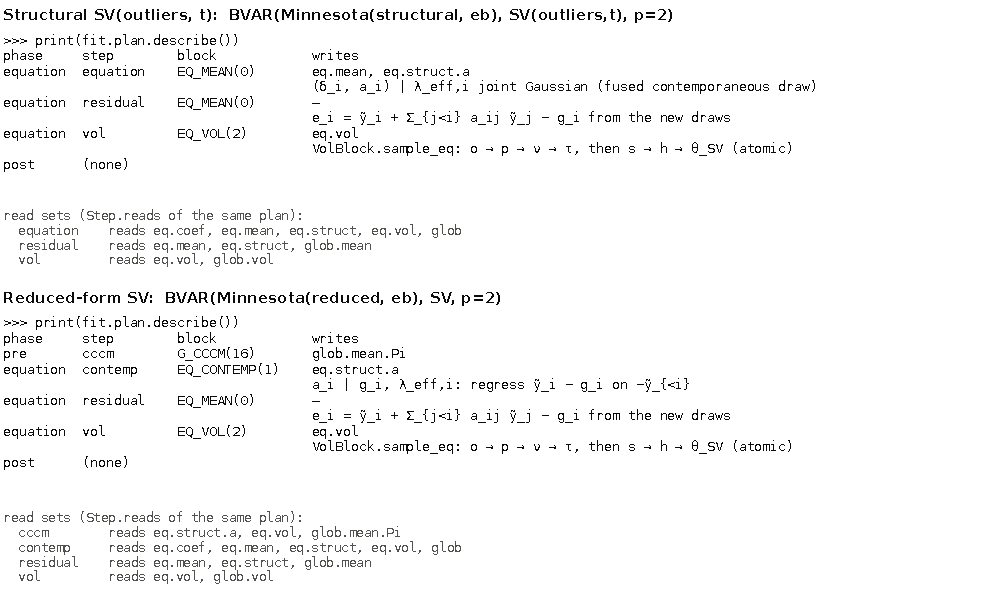
\includegraphics[width=\linewidth]{figures/fig_plan.pdf}
\caption{The Gibbs plan as data: the output of \code{fit.plan.describe()} (each step's block and
write set) for a structural SV(outliers, $t$) model and a reduced-form SV model, fitted to the
simulated data of \cref{lst:Lst2}, followed by each step's declared read set
(\code{Step.reads}). The mixture indicators are local to
the \texttt{vol} step, so no step runs between the indicators and $h$.}
\label{fig:FigC1}
% [V] src/rai_bvar/engines/mcmc/plan.py (describe() l.91-103 prints block and write set); generated by docs/paper/figures/make_fig_plan.py
\end{figure}

\begin{table}[!htbp]
\centering\footnotesize
\caption{The predictive contract: fields of \code{ForecastResult}, which wraps an
\code{xarray.Dataset}. The accelerator variables are carried by MCMC forecasts only, are ignored by
\code{check_structure} and by every consumer, and are never contract fields.}
\label{tab:TabC1}
% [V] src/rai_bvar/forecast/result.py:1-19, :96-162 (62d15f6); tests/contract/test_forecast_contract.py,
% tests/contract/test_forecast_contract_mcmc.py (12 MCMC compositions, tests/mcmc/forecast/mcmc_fits.py:128-141);
% lag_coefs added in b9c66c0 (D-34); checked against a live ForecastResult by docs/paper/figures/tab_contract.py
\begin{tabular}{@{}p{0.20\linewidth}p{0.28\linewidth}p{0.45\linewidth}@{}}
\toprule
Field & Dimensions & Meaning \\
\midrule
\code{paths} & (chain, draw, horizon, variable) & joint simulated paths on the transformed scale; each slice is one path from one parameter draw \\
\code{paths_level} & same & pathwise inverse of the tcodes to raw levels (\cref{tab:tcodes}) \\
\code{cond_mean} & same & $m_{s,h}$: mean of $y_{T+h}$ given the draw, the simulated path to $T + h - 1$ and $\lambda_{T+h}$ \\
\code{cond_chol} & (\dots, variable, variable\_) & $L_{s,h}$: lower-triangular factor of the conditional covariance \\
attrs (all engines) & --- & \code{origin}, \code{freq}, \code{model}, \code{engine}, \code{spec}, \code{spec_hash}, \code{tcodes}, \code{seed}, \code{converged}, \code{warnings}, \code{rai_bvar_version}; analytic adds \code{mh_seed} \\
attrs (MCMC) & --- & \code{ordering}, \code{n_chains}, \code{mixture}, \code{exact}, \code{transitory}, \code{outlier_K}, \code{t_scale}, \code{fseed} and the fit's reproducibility metadata (\cref{app:repro}) \\
\midrule
\multicolumn{3}{@{}l}{\emph{Accelerator variables (MCMC only; not contract fields)}} \\
\code{cond_A}, \code{cond_scale} & (chain, draw, variable, variable\_), (chain, draw, horizon, variable) & $A$ and the effective scales, so that $\mathrm{cond\_chol} = A^{-1}\operatorname{diag}(\mathrm{cond\_scale})$; O($n^2$) factored densities \\
\code{cond_scale_persistent}; \code{log_p}, \code{log1m_p}, \code{nu} & (chain, draw, horizon, variable); (chain, draw, variable) & inputs of the opt-in transitory Rao--Blackwellisation (\code{rb_transitory=True}) \\
\code{lag_coefs} & (chain, draw, lag, variable, variable\_) & $A_l$ of each draw, used by the path-integrated estimator at $h > 1$ (D-34) \\
\midrule
\multicolumn{3}{@{}p{0.95\linewidth}@{}}{\emph{Invariants.} $L^{-1}(\mathrm{paths} - \mathrm{cond\_mean})$ is iid $\mathrm{N}(0, I)$; draws are joint across horizons and variables; stacking (chain, draw) gives the shape (draws, $H$, $n$) in chain-major order. Analytic forecasts carry no \code{ordering} attribute; their ordering is the \code{variable} coordinate.} \\
\bottomrule
\end{tabular}
\end{table}

The contract tests run for every registered analytic model and for 12 MCMC compositions:
structural $\times$ \{SV, SV(outliers), SV($t$), SV(outliers, $t$), SV(rw), Constant(ig),
Constant(iw), Constant(iw\_equivalent)\} and reduced $\times$ \{SV, SV(outliers), Constant(ig),
Constant(iw\_equivalent)\}.
Reduced $\times$ SV($t$), reduced $\times$ SV(rw) (the primary arm of the replication) and reduced
$\times$ SV(outliers, $t$) are not in this list.
% [V] tests/mcmc/forecast/mcmc_fits.py:128-141 (re-run, dossier 02 section 0.1); unchanged in the committed
% tree at d58c9ef
\todo{TODO 3: row~18, \code{reduced_sv_rw} (reduced form $\times$ SV(rw)), and a \code{reduced-SV(rw)} contract fit were committed in 7f410dc, after the acceptance commit c823d20; the SV(rw, $t$) variant is still not covered. If the release commit includes it, update this list, \cref{app:sbc} and the main-text caveats.}

\clearpage

% -------------------------------------------------------------------------------------
\section{Validation detail}\label{app:validation}
% -------------------------------------------------------------------------------------

This appendix gives the configurations, statistics and run records behind
\cref{sec:validation}.
The tables here are to be generated on the release commit, from the JSON records that the Geweke,
SBC and mutation tests write when \code{RAI_BVAR_VALIDATION_RECORD} points to a directory and, for the
tiers without such a hook, from the test run's output (\cref{app:repro}).
% [V] record hooks only in tests/geweke/test_geweke_compositions.py, tests/sbc/test_sbc_compositions.py,
% tests/mutation/test_mutants.py (git grep RAI_BVAR_VALIDATION_RECORD at d58c9ef)
Where a number below was reproduced on an earlier commit, the commit and the machine are stated.
\todo{TODO 7: record G-small, G-full, SBC, composition-level B, the \code{exact=False} rows,
\code{parity_long}, the analytic twins and the mutation suite on the release commit (Apple M5 Max and
x86-64 Linux) and commit the JSONL files.}

\subsection{Geweke tests at the per-PR size}\label{app:geweke-small}

The G-small configuration runs $C = 1000$ independent successive-conditional chains of $M_c = 100$
sweeps, each started at a prior draw with no burn-in, against $M_1 = 2\times10^5$ iid
marginal-conditional draws, with family level $\alpha = 10^{-3}$, $t_{C-1}$ critical values and the
sequential wrapper of \citet{gandy2021unit} with $k = 3$ stages and multiplier $\Delta = 4$.
The test data have $T_{\mathrm{eff}} = 20$, never a multiple of the 32-row bucket, $n = 2$ in
structural and $n = 3$ in reduced form (with the design table's overrides: $n = 3$ for row 205 and
$n = 1$ for the univariate row 17), $p = 1$ and an intercept.
% [V] src/rai_bvar/validation/joint.py docstring and _COMPOSITIONS (n overrides)
% [V] tests/geweke/test_geweke_compositions.py (SEED_SMALL = 20261022; test_g_small asserts T_eff % 32 != 0)
\cref{tab:TabD1} gives the result for each of the 15 per-PR compositions.
On commit 62d15f6 (Apple M5 Max) every composition passed: the largest final-stage $|z|$ was 3.03
against critical values of 4.10--4.50; row 201 went to a second, fresh and larger stage after a
first-stage Bonferroni $q$ of 0.0012 ($|z| = 4.21$ on a log-scale data autocorrelation) and passed
there with $q = 1.0$; and the minimum relative numerical efficiency per composition was 0.008--0.129.
% [V] reproduced twice at 62d15f6 on Apple M5 Max (dossier 04 section 6.6 and its fact-check);
% deterministic for fixed code and seed on that machine, not a cross-machine reproduction; [REL]
The sequential design bounds the probability of a false rejection by
$\sum_i \gamma^{i-1}\beta_i = \alpha$, with $\beta_1 = \alpha/k$, $\gamma = \beta_1^{1/k}$ and
$\beta_{i+1} = \beta_i/\gamma$; a stage fails if $q_i \le \beta_i$, passes if $q_i > \gamma +
\beta_i$, and otherwise hands the decision to a new, independent experiment, enlarged once by
$\Delta$.
At the per-PR settings $\gamma = 0.0693$ and $\beta = (3.33\times10^{-4}, 4.81\times10^{-3},
0.0693)$, so a correct sampler is rerun at four times the size with probability at most about
7\%.
% [V] src/rai_bvar/validation/sequential.py docstring; tests/validation/test_sequential.py;
% [R] the expected extra effort (about 30%): docs/phase2/06_validation_geweke_sbc.md section 4.6

\begin{table}[!htbp]
\centering\small
\caption{G-small Geweke results for the 15 per-PR compositions: number of test functions
$G$, $t_{C-1}$ critical value, maximum $|z|$ and its argument, Gandy--Scott stage and Bonferroni
$q$, minimum relative numerical efficiency, and time. Generated from \code{geweke.jsonl}
(\code{pytest tests/geweke -m "geweke and not slow"}) on the release commit.}
\label{tab:TabD1}
% [REL] docs/paper/data/release/geweke.jsonl; generated by docs/paper/figures/tab_geweke.py;
% cross-check against dossier 04 section 6.6 (62d15f6)
\InputIfFileExists{figures/tab_geweke.tex}{}{\todo{Generate with \code{tab_geweke.py} from the
release \code{geweke.jsonl}.}}
\end{table}

\subsection{Geweke test functions and the finite-variance rule}\label{app:geweke-functions}

The test functions of every composition are drawn from fixed families: every scalar parameter;
latent states at fixed dates ($h_{i,0}$, $h_{i,1}$, $h_{i,\lceil T/2\rceil}$, $h_{i,T}$) and the path
means $\operatorname{mean}_t h_{i,t}$ and $\operatorname{mean}_t |h_{i,t}|$; squares where their
variance is finite; cross-products within blocks
($a_{ij}\gamma_{i,(\mathrm{lag}\,1, j)}$, $\mu\phi$, $\phi\sigma$, $p\,N_1$, $\nu\cdot\operatorname{mean}
\log\tau$); cross-equation products of reduced-form coefficients; the exact log-likelihood given the
latent states and the log prior density $\log p(\theta)$; the standardised residual sums $\sum_t
e_{it}^2/\lambda_{it}$; and data functions.
% [V] DESIGN section 9.5; src/rai_bvar/validation/testfns.py docstring; reference.py _sv_dates (h0, h1, hmid,
% hT, mean_h, mean_abs_h); G-small asserts len(spec.names) >= 20
The number of functions per per-PR composition ranges from 22 (univariate SV) to 134 (reduced form
with SV and outliers).
% [V] reproduced at 62d15f6 (dossier 04 section 6.6)
Geweke's statistic is asymptotically normal only if $\operatorname{var}g(\theta, y) < \infty$
\citep{geweke2004getting}.
Under the SV test prior $\mathrm{E}[y^2] = \mathrm{E}[e^h]$ is infinite, because $\sigma^2$ has a
$\chi^2$ tail and $\phi$ has prior mass near 1; under $\mathrm{IG}(3, 2)$ the variance of
$\lambda^2$ is infinite; and with Student-$t$ errors $\mathrm{E}[y^{2k}]$ is finite only for $\nu >
2k$.
The rules adopted are therefore: under SV only log-scale or bounded data functions
($\operatorname{mean}_t\log y_t^2$, sample correlations, first autocorrelations,
$\operatorname{mean}_t\tanh y_t$); $\log\lambda$ in place of $\lambda^2$; and a Constant test prior
$\mathrm{IG}(5, 4)$.
Each reference function carries a finite-variance flag.
% [R] heavy-tail simulation (batch means of mean y^2 from 2.3 to 5.2e3; mean log y^2 -1.27 in every batch):
% docs/phase2/06_validation_geweke_sbc.md section 3.4 (script not committed); [V] reference.py flags
The test priors are proper and tight, $M \ne 0$ so that D3 centring is exercised, $a_{ij} \sim
\mathrm{N}(0, 0.7^2)$, the outlier probability is $\mathrm{Beta}(2, 18)$ so that outliers occur at
$T = 20$, $\nu \in \{5, \dots, 12\}$, and the in-window recomputation of hyperparameters is off, so
that no hyperparameter depends on $y$.
% [V] src/rai_bvar/validation/joint.py docstring l.13-29; DESIGN section 9.2
The size of the test needs only that the sweep leaves the posterior invariant: a chain started at a
prior draw is stationary from its first sweep under the null, and its mean is an unbiased estimate of
$\mathrm{E}_p[g]$; ergodicity affects only power.
% [R] docs/phase2/06_validation_geweke_sbc.md section 3.1 (argument); TODO 15 for any attribution
At $G = 100$ and $\alpha = 10^{-3}$ the normal critical value would give an actual size of
$1.64\times10^{-3}$ at $C = 200$ and $1.11\times10^{-3}$ at $C = 1000$, which is why the $t_{C-1}$
quantile is used.
% [R] docs/phase2/06_validation_geweke_sbc.md section 3.2 (computation recorded there)

\subsection{G-full, the approximate rows, Tier B and SBC}\label{app:sbc}

G-full uses $C = 4000$, $M_c = 500$, $M_1 = 10^6$ and $\alpha = 10^{-2}$ at $n = 3$, $p = 2$ and
$T_{\mathrm{eff}} = 50$ (rows 14--16: $n = 2$; row 17: $n = 1$); the eleven \code{exact=False} rows
(the auxiliary-mixture sampler) are recorded but do not gate, because that sampler targets the
mixture approximation rather than the exact posterior; only a non-finite test function, which is a
bug whatever the approximation, fails them.
% [V] tests/geweke/test_geweke_compositions.py::test_pr_rows_are_the_design_rows, ::test_g_full_inexact_recorded
Composition-level Tier B consists of block-conditional SBC ($N = 200$, $L = 99$) of every exact-draw
block, with ranks of the block's coordinates and of the exact log-likelihood, and one-block invariance
($N = 1000$ joint draws, $L = 20$ applications of the live blocks, two-sample Kolmogorov--Smirnov tests)
for Metropolis--Hastings, ASIS and Gibbs-scan blocks; its 43 tests run weekly, while each kernel
suite runs its own Tier~B per PR.
% [V] tests/sbc/test_block_tier.py docstring l.4-28 (pytestmark slow)
SBC uses $N = 1000$ replications, $L = 99$ kept draws, burn-in 300, a pilot of 1000 sweeps,
$t_{\max} = 200$ and $\alpha = 10^{-2}$ for the 22 compositions, inside the same sequential wrapper.
% [V] tests/sbc/test_sbc_compositions.py docstring l.1-11 (committed tree, d58c9ef); [R] t_max = 200 (docstring l.13-21)
\todo{TODO 3: row~18, \code{reduced_sv_rw} (reduced form $\times$ SV(rw)), and a \code{reduced-SV(rw)} contract fit were committed in 7f410dc, after the acceptance commit c823d20; the SV(rw, $t$) variant is still not covered; NOTES item 6 records that it passes the ESS rule only with a per-row $t_{\max}$ of 400. If the release commit includes it, update the composition count and the cap here.}
Each replication draws $(\tilde\theta, \tilde y)$ from the joint model, applies only the data filter
$\operatorname{finite}(\tilde y) \wedge \max|\tilde y| < 10^3$, runs a pilot chain from an
independent prior draw, sets its thinning to $t_i = \min(\lceil 2\,\mathrm{IAT}_i\rceil,
t_{\max})$ with the Geyer initial-monotone IAT \citep{geyer1992practical} of the quantities and of
their tail indicators, and then keeps $L$ draws from a fresh chain; ranks are uniform conditionally
on $\tilde y$, so data-dependent thinning preserves uniformity.
Uniformity is tested with the $\gamma$ statistic of \citet{sailynoja2022graphical}, whose null
distribution is computed exactly by a forward recursion that accumulates the mass leaving the
interior at each step, so that $p$-values in the far tail keep their relative accuracy.
% [V] src/rai_bvar/validation/sbc.py, uniformity.py; tests/validation/test_uniformity.py
The quantities include the parameters, $h$ at fixed dates and its path means, the total and per-equation
log-likelihood, $\log p(\theta)$ and the predictive unknowns $h_{T+1}$ and $y_{T+1}$ through the
production forecast core; data-dependent quantities are needed because a ``posterior'' equal to the
prior passes SBC on every data-free quantity \citep{modrak2025simulation}.
% [V] tests/sbc/test_sbc_compositions.py::test_quantity_selection, ::test_truth_and_forecast_core_are_the_same_map

\emph{The ESS erratum.}
The design asked for a per-replication thinned ESS of at least $0.8L$ in 99\% of replications.
With $L = 99$ kept draws that cannot be certified for a single replication: even with iid draws the
Geyer ESS of the kept draws reaches $0.8L$ only in about three replications out of four.
The per-replication ESS is therefore predicted from the pilot IAT with an AR(1) form, $\rho_i =
(\mathrm{IAT}_i - 1)/(\mathrm{IAT}_i + 1)$ and $\mathrm{ESS}_i = L(1 - \rho_i^{t_i})/(1 +
\rho_i^{t_i})$, which is at least $0.96L$ whenever $t_i$ is not capped, and a second gate requires
the replication-pooled ESS of the kept draws, computed from autocovariances of ECDF indicators pooled
over replications (a level is used only when Kish's effective number of replications is large
enough), to be at least $0.8L$ for every quantity.
% [V] design change: DESIGN section 9.6 erratum; src/rai_bvar/validation/sbc.py docstring l.24-54;
% [R] the "about 76%" and "0.836 L" figures are docstring-only (TODO 25)
\todo{TODO 25: commit a small test for the 76\% and $0.836L$ figures, or keep them out.}
\cref{tab:TabD3} collects the G-full, \code{exact=False}, composition-level B and SBC records.
No committed record of these runs existed at 62d15f6; the only committed numbers are those that the
repository notes record for row 205 (G-full 2.76, SBC minimum $p$ 0.018).
% [R] NOTES 13 (dossier 04 sections 6.7, 7.6); [REL] geweke.jsonl (tiers G-full, G-full-inexact), sbc.jsonl;
% composition-level B has no record hook yet (TODO 7)

\begin{table}[!htbp]
\centering\small
\caption{G-full, the recorded \code{exact=False} rows, composition-level Tier~B and full SBC per
composition: maximum $|z|$ or minimum $p$, stages, ESS gates and the number of replications
at $t_{\max}$. Generated on the release commit.}
\label{tab:TabD3}
% [REL] docs/paper/data/release/geweke.jsonl (tiers G-full, G-full-inexact), sbc.jsonl; composition-level B needs a record hook (TODO 7); docs/paper/figures/tab_geweke_full_sbc.py
\InputIfFileExists{figures/tab_geweke_full_sbc.tex}{}{\todo{Generate with
\code{tab_geweke_full_sbc.py} from the release records; until then no G-full or SBC result other than
row 205 is stated.}}
\end{table}

\subsection{Analytic twins and exact oracles}\label{app:twins}

\cref{tab:TabD4} lists the twins A1--A7 with their oracle, statistic, tolerance, negative
control and cadence.
Two methodological details matter for reading it.
First, the twins compare quantiles in CDF form: each exact quantile $x_q$ is tested by $z =
(\hat F_{\mathrm{MCMC}}(x_q) - q)/\sqrt{\mathrm{MCSE}^2(\hat F) + q(1-q)/N_{\mathrm{ref}}}$, with
the indicator's own ESS.
To first order this equals the quantile-MCSE test, but it avoids the density estimate of the
order-statistic MCSE, whose noise made the usual statistic heavy-tailed at $n = 20$; the decision
rule is $|z| \le \max(4, z_{\mathrm{Bonf}})$ at family level $10^{-2}$.
% [R] tests/analytic/test_mcmc_twin.py docstring "Comparison" (the -4.99 example is withheld, TODO 25);
% [V] the comparison is implemented by the committed tests
Second, the twins carry negative controls whose rejection is part of the test: for example, A2
rejects an NIW posterior with one extra degree of freedom (a change of about 1.5\% in $\Sigma$), and
A5 rejects an inverse-gamma shape off by $\frac12$ (about 1.6\% in $\mathrm{E}[\lambda_i]$).
% [V] tests/analytic/test_mcmc_twin.py::test_a2_rejects_a_slightly_wrong_posterior;
% tests/analytic/test_mode1_quadrature.py::test_a5_rejects_a_slightly_wrong_posterior
The quadrature oracle of A5 checks itself on every call (doubling the rule and widening the interval
changes nothing above $10^{-10}$), and with a $\lambda$-scaled prior on all coordinates it must
reproduce the closed form of \citet{chan2022asymmetric}.
% [V] tests/analytic/test_mode1_quadrature.py docstring; ::test_quadrature_reproduces_the_structural_nig_closed_form
The twins are also the tier that caught a missing term the dense oracles of the coefficient step did
not: in Mode~II with dummy rows, the $\lambda$ step must count the rows (\cref{app:dummies}).
% [R] NOTES 12 (hand injection; the quantile count is withheld until TODO 24)

\begin{table}[!htbp]
\centering\small
\caption{Analytic twins and exact oracles A1--A7: oracle, statistic and tolerance, negative
control and its measured power, cadence, and result on the release commit.}
\label{tab:TabD4}
% [V] tests/analytic/test_mcmc_twin.py, test_mode1_quadrature.py, test_structural_nig.py;
% tests/mcmc/blocks/test_sv_toy_quadrature.py, swa_oracle.py; [REL] docs/paper/data/release/twins.xml
\InputIfFileExists{figures/tab_twins.tex}{}{\todo{Generate with \code{tab_twins.py} from the release
junit XML.}}
\end{table}

\subsection{Parity with independent implementations}\label{app:parity}

Parity runs both implementations on the same committed datasets with one parameter set from which
both sides' settings are derived, and compares the 5, 25, 50, 75 and 95\% quantiles with $z =
(\hat q_{\mathrm{ours}} - \hat q_{\mathrm{ref}})/\sqrt{\mathrm{mcse}^2_{\mathrm{ours}} +
\mathrm{mcse}^2_{\mathrm{ref}}}$, passing if $|z| \le \max(4, z_{1 - 0.01/(2m)})$ over the $m$
comparisons; the MCSE is the larger of the quantile MCSE of \citet{vehtari2021rank} and a
batch-quantile MCSE.
% [R] tests/parity/SV_PARAMETRIZATION.md section 2 (l.73-81); [V] tests/parity/test_stochvol.py
\cref{tab:TabD2} summarises the rows used as evidence in this paper; the parametrisation notes
in \code{tests/parity/} record every convention that had to be matched.
\begin{itemize}
\item \emph{Analytic engine.} R \pkg{BVAR} 1.0.5 \citep{kuschnig2021bvar} and the Bank of England
\pkg{bvar} 0.3.5 \citep{labonne2026bvar}. The tests assert log marginal likelihoods at fixed
hyperparameters to a relative tolerance of $10^{-8}$; the recorded agreement is below $10^{-11}$ for
\pkg{BVAR} in the exact cases and at most $1.5\times10^{-11}$ for the Bank of England package.
Posterior moments are tested to a relative tolerance of $10^{-8}$ (the largest recorded deviation
is $6\times10^{-9}$), empirical-Bayes modes to $10^{-3}$, and Metropolis--Hastings and forecast
quantiles within Monte Carlo error.
% [R] BVAR_PARAMETRIZATION.md section 12; BOE_BVAR_NOTES.md section 14 (dossier 04 section 10.3)
% [V] tests/parity/test_r_bvar.py (147 IDs), test_boe_bvar.py (38 IDs); [R] BVAR_PARAMETRIZATION.md section 12,
% BOE_BVAR_NOTES.md section 14
\item \emph{Univariate SV.} \pkg{stochvol} 3.2.1 \citep{kastner2016dealing,hosszejni2021modeling}
against \code{ZeroMean} $\times$ SV with $n = 1$, on the main and default-prior rows of four
datasets: maximum $|z|$ 1.63--2.59 at the per-PR size and 1.64--3.57 at the size of the weekly tier, against a bound of 4.00.
% [R] tests/parity/SV_PARAMETRIZATION.md section 6 table (machine label under review, TODO 8); tests committed
\item \emph{Standardised Student-$t$ SV.} The exit criterion for this sampler is an exact posterior
obtained by self-normalised importance sampling on a four-observation problem, against which the
maximum $|z|$ is 1.83. A small problem with an exact posterior is an oracle that does not depend on
any other implementation.
% [V] tests/parity/test_stochvol.py::test_sv_t_matches_the_exact_importance_sampling_posterior
\todo{TODO 13: re-test the third-party Student-$t$ and sign-fold observations on the current releases
and contact the maintainers before any statement about another package's sampler; until then this
appendix states none.}
\item \emph{Reduced form.} \pkg{bayesianVARs} \citep{gruber2026bayesianvars} could not be built in the
test environment (no Fortran compiler), so no finding about it is stated. The exit criterion was met
against a substitute: an exact system-wide Gibbs sampler written in R in \pkg{rai-bvar}'s own
conventions ($\operatorname{vec}\Pi \mid A, \Lambda$ jointly, $A$ rows by regression, SV by one sweep
of \pkg{stochvol}'s sampler at offset 0, or $\lambda_i \mid e$ inverse gamma), which gives maximum
$|z|$ 2.76, 3.45 and 3.56 against bounds of 4.05--4.51.
% [R] tests/parity/SV_PARAMETRIZATION.md sections 4 and 6; tests/parity/test_bayesianvars.py committed
\end{itemize}
Parity does not establish everything: there is no external VAR-level oracle for structural Mode~I
$\times$ SV, and exact mode has no external oracle beyond the reweighted \pkg{stochvol} rows.

\begin{table}[!htbp]
\centering\small
\caption{Parity summary: oracle and version, rows, statistic, bound, and maximum $|z|$ or
relative tolerance.}
\label{tab:TabD2}
% [R] tests/parity/SV_PARAMETRIZATION.md section 6; BVAR_PARAMETRIZATION.md section 12;
% BOE_BVAR_NOTES.md section 14; [REL] docs/paper/data/release/parity.jsonl (pytest -m parity_long)
\InputIfFileExists{figures/tab_parity.tex}{}{\todo{Generate with \code{tab_parity.py}; neutral
wording only (TODO 13).}}
\end{table}

\subsection{The mutant catalogue}\label{app:mutants}

A mutant is injected only through a production seam: a named kernel internal overridden through
\code{compose(static, overrides=...)}, the volatility slot, the sampler's prior arrays, the
observables simulator, or the configuration.
A tier catches a mutant when its decision rule fails on the mutant and passes on the unmutated
control with common seeds; for a U check, the mutant's error must exceed the tolerance and the
control's must not, at the same joint draw.
\code{test_registry} requires every mutant to have at least one confirmed catching tier, and a
mutant caught by none blocks the release.
% [V] tests/mutation/mutants.py docstring l.1-45, run_tier; tests/mutation/test_mutants.py
The U checks use a tolerance of $10^{-8}$ (M8 and M11: $10^{-12}$; M12: $10^{-4}$; M15:
$10^{-10}$); the B checks are the block SBC of $\pi_0$ or one-block invariance of the volatility
block; G is \code{geweke_sequential} at G-small; S is a short SBC ($N = 200$, four times that after
stage 1, $L = 99$, burn-in 100, pilot 300, $t_{\max} = 30$).
% [V] tests/mutation/mutants.py _ALL (l.767-826), sbc_check (l.714-726)
The mutant and control statistics are in \cref{tab:Tab7}; below, each entry gives the seam,
the error as a mathematical statement, its source where it has one, and the catching tiers.
\begin{description}\small
\item[M1] (\code{cccm_core}; reduced Constant.) $\pi_j$ is drawn from equation $j$ alone, the
triangular step of \citet{carriero2019large}, instead of the corrected full conditional
\citep{carriero2022corrigendum}. Caught by U, B (through the log-likelihood rank) and G;
one-block invariance of the whole scan does not catch it (recorded; \cref{app:ccm-flat}).
\item[M2] (volatility slot, \code{exact=False}; structural SV.) Stale indicators: $s$ is carried
across sweeps and drawn after $h$, the order of Algorithm~1 of \citet{primiceri2005time} corrected
by \citet{delnegro2015time}. Caught by G.
\item[M3] (\code{JointSpec(fresh_latents=True)}; structural SV.) The observables simulator draws
fresh latent states instead of using the current ones, the simulator error of
\citet{geweke2004getting}. Caught by G.
\item[M4] (\code{tau_conditional}; structural SV($t$).) $\tau_t \mid \cdot$ has shape $\nu/2$ instead of
$(\nu + 1)/2$. Caught by U and G.
\item[M5] (sampler prior arrays; structural SV.) $B_\sigma$ is doubled in the sampler only, so the
sampler's prior differs from the model's. Caught by G.
\item[M6] (\code{nc_fold}; univariate SV.) The non-centred step takes $|\sigma|$ without flipping
$\tilde h$, which is not measure-preserving (\cref{app:exact-sv}). Caught by U and G.
\item[M7] (\code{nc_accept}, with the one-component table COARSE1 in mutant and control; univariate
SV.) The non-centred move is accepted without the $w$-correction in exact mode. With OCSN-10 the
missing correction is too small to see at test sizes. Caught by U and G.
\item[M8] (\code{structural_gamma}; structural Constant.) D3 centring is dropped, $\gamma_i =
\delta_i$. Caught by U, G and S.
\item[M9] (\code{outlier_logits}; structural SV(outliers).) The outlier pmf omits the factor
$1/k$. Caught by U and G.
\item[M10] (\code{p_conditional}; structural SV(outliers).) $p \mid o \sim \mathrm{Beta}(a_p + N_1,
b_p + T)$ instead of $b_p + T - N_1$. Caught by U and G.
\item[M11] (\code{indicator_logits}; auxiliary sampler.) The indicator pmf omits $v_j^{-1/2}$.
Caught by U, B and G under \code{exact=False}; in exact mode it is not a bug, and the G check passes
there (recorded).
\item[M12] (\code{mixture_table}; auxiliary sampler.) The effective component means are shifted by
$-1.2704$ twice. Caught by U, B and G under \code{exact=False}; not a bug in exact mode (recorded).
\item[M13] (\code{constant_conditional}; structural Constant.) The inverse-gamma shape uses
$T_{\mathrm{pad}}$ instead of $T_{\mathrm{eff}}$. Caught by U and G.
\item[M14] (\code{contemp_conditional}; reduced Constant.) The $A$-row regression uses $+u_{<j}$
instead of $-u_{<j}$. Caught by U and G.
\item[M15] (\code{nc_step}; univariate SV.) The ASIS map omits the rescaling of $\tilde h$.
Caught by U, B and G.
\item[M16] (configuration, \code{exact=False}; univariate SV.) Offset $c = 0.1$ at $\lambda \approx
0.01$ (prior level centred at $\log 0.01$) against a control offset of $10^{-12}$. In exact mode a
large offset is not a bug, so the mutant is defined for the auxiliary sampler only. Caught by G.
\item[M17] (\code{linear_conditional}; structural Constant with dummies.) Mode~I SOC/SUR rows are
weighted by the current $1/\lambda_i$ instead of the fixed $1/\bar\sigma_i^2$. Caught by U and G;
its G control runs on the dense eigen path (control statistic 1.94; 2.44 on the
\code{cholesky_const} path).
\item[M18] (\code{cccm_core}; reduced Constant with dummies.) The SOC/SUR rows are dropped from the
CCCM step. Caught by U and G.
\end{description}
% [V] catchers and seams: tests/mutation/mutants.py _ALL; 37/37 reproduced at 62d15f6 on Apple M5 Max
% (dossier 04 section 11.2, re-run by its fact-check); [R] M1-M16 x86-64 Linux re-run and M17-M18 "4 passed":
% mutants.py EVIDENCE header (machine labels to fix, TODO 8); [REL] mutation.jsonl, mutation_x86.jsonl
Coverage is U 14 of 18, G 18 of 18, B 4 (every mutant with a registered B check) and S 1, which is
37 mutant $\times$ tier checks.
% [V] reproduced at 62d15f6 (dossier 04 section 11.2)
The four mutants without a U check, M2, M3, M5 and M16, carry \code{u_check=None} in the registry:
they are errors of step order, of the simulator, of a sampler--model prior mismatch and of a model
approximation, and no deterministic identity is registered for them.
Whether an identity could detect them is not tested; for M5, a density-ratio identity of the
$\sigma^2$ step against the model prior is a plausible detector.
% [V] tests/mutation/mutants.py _ALL (M2 l.771-773, M3 l.774-776, M5 l.780-782, M16 l.815-818)
The design expected U catches for nine mutants; the suite confirmed fourteen, and G for all eighteen.
% [V] DESIGN section 9.7 expected-catcher column vs _ALL
The independent x86-64 review also caught four further hand-injected dummy-row errors (Mode~II rows
weighted $1/\bar\sigma^2$, rows counted twice in the $\lambda$ step, CCCM rows weighted by
$(\Sigma^{-1})_{jj}$, a fixed-factor weight $2w$); these are not registered mutants.
% [R] NOTES 15

\cref{fig:FigD1} shows, for each mutant and tier, the mutant's statistic relative to the
tier's decision threshold, and \cref{fig:FigD2} places the G statistics of the mutants against
the per-composition controls (G-full rows of the validation record and the mutation suite's
G-small controls).
Statistics agree across machines to two or three significant figures (for M2, 702 and 705 for the
mutant, 2.47 and 2.48 for the control); they are not expected to agree bitwise across platforms.
% [V] M2 705 / 2.48 reproduced at 62d15f6 (Apple M5 Max); [R] 702 / 2.48 and 705 / 2.47 from EVIDENCE

\begin{figure}[!htbp]
\centering
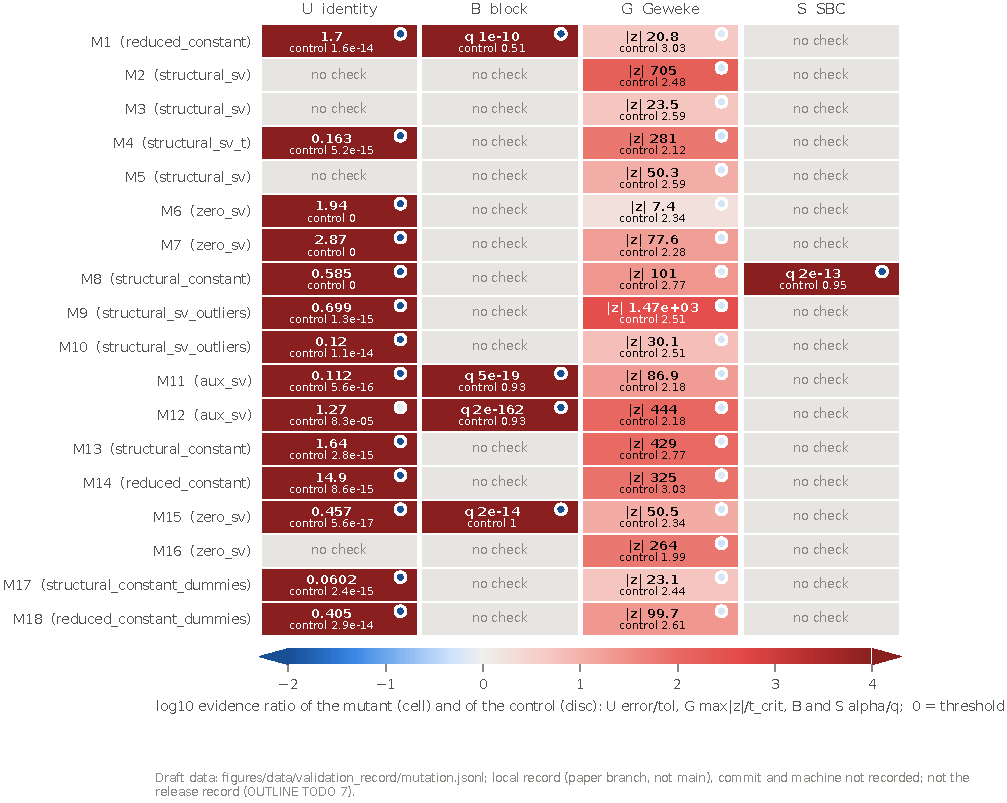
\includegraphics[width=0.85\linewidth]{figures/fig_mutation_heatmap.pdf}
\caption{Mutation power: mutants M1--M18 $\times$ tiers U, B, G, S. Cell colour is
$\log_{10}$ of the mutant's statistic divided by the tier's decision threshold; a marker shows the
control; grey means that no check is registered.}
\label{fig:FigD1}
% [REL] docs/paper/data/release/mutation.jsonl (+ mutation_x86.jsonl); docs/paper/figures/make_fig_mutation_heatmap.py
\end{figure}

\begin{figure}[!htbp]
\centering
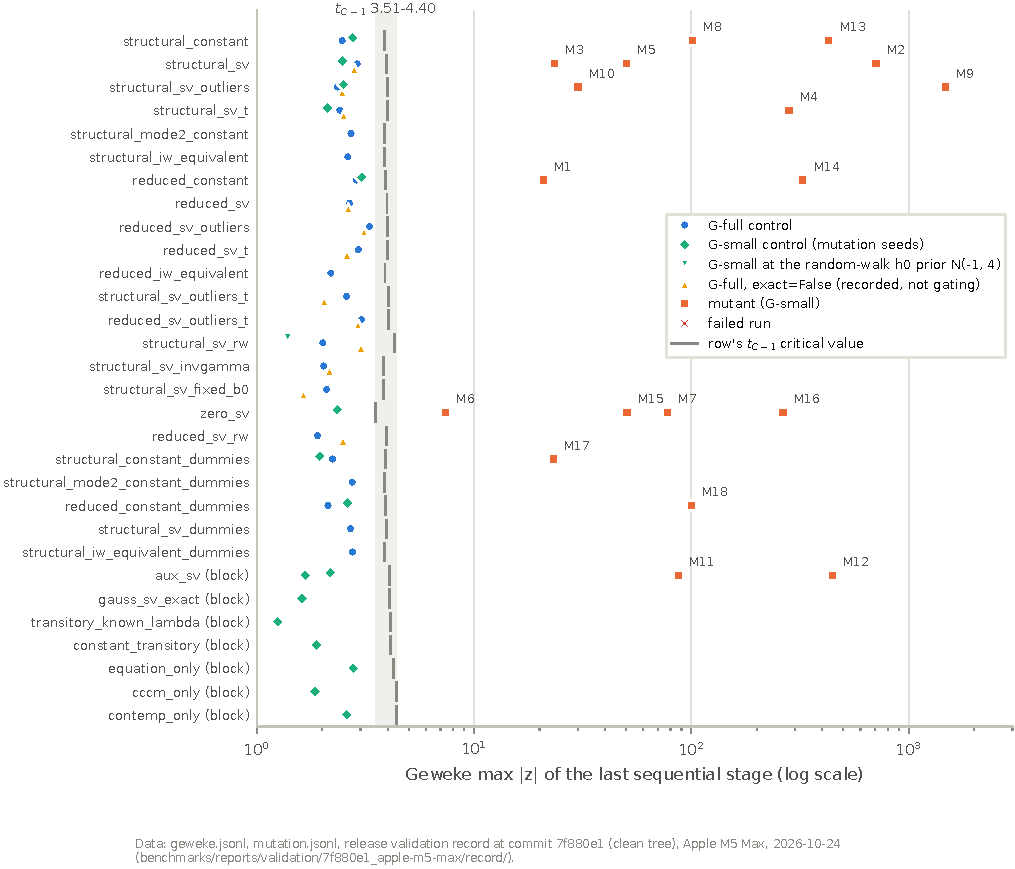
\includegraphics[width=0.85\linewidth]{figures/fig_geweke_dots.pdf}
\caption{Geweke maximum $|z|$ per composition for the unmutated samplers (G-full rows and the
recorded \code{exact=False} rows of the validation record, and the mutation suite's G-small controls
at the mutation seeds) against the $t_{C-1}$ critical band, with the mutants' G statistics overlaid on a
logarithmic scale; failed runs are drawn as crosses.}
\todo{TODO 7: this draft figure is drawn from local, uncommitted records
(\code{docs/paper/figures/data/validation_record/}) that carry no commit or machine field and hold
no registered G-small rows; in them the G-full row of \code{reduced_sv} failed with non-finite test
functions (seed 20261023), which is either the float64 failure that 3d3f51b fixed (a stale record) or
a regression; the record cannot say which. Establish their provenance or redraw from the release
records.}
\label{fig:FigD2}
% [REL] docs/paper/data/release/geweke.jsonl (tiers G-small, G-full), mutation.jsonl; docs/paper/figures/make_fig_geweke_dots.py (--geweke/--mutation select the release records)
\end{figure}

\subsection{Runtime convergence diagnostics}\label{app:diagnostics}

The convergence flag is computed by in-repository NumPy code: rank normalisation with normal scores
$(r - 0.375)/(S + 0.25)$, split chains, R-hat as the maximum of the bulk and folded versions
\citep{vehtari2021rank}, ESS with Geyer's initial positive and monotone sequence truncation
\citep{geyer1992practical}, and tail ESS, mean ESS and the MCSE of means and quantiles.
% [V] src/rai_bvar/diagnostics.py (_rank_normalise l.23-25, rhat l.37, _geyer_ess l.209)
The diagnostics are tested against reference values from ArviZ 0.23.4 and \pkg{arviz-stats} 1.3.3
\citep{kumar2019arviz}, which agree with each other to the last digit on every case and are
hard-coded in the tests (ArviZ is not a dependency), to a relative tolerance of $10^{-10}$; against
stationary Gaussian AR(1) chains with closed-form IATs, including the indicator IAT; and by
statistical bounds calibrated over 30 seed sets.
% [V] tests/mcmc/diagnostics/test_diagnostics_ext.py::test_matches_arviz, ::test_ar1_known_autocorrelation_times,
% ::test_mcse_coverage_over_many_replications, ::test_tail_ess_sees_what_bulk_ess_misses
The gate is decided by the primary monitor set only: at $n = 20$ it has 41 quantities for Constant,
101 for SV, 61 for random-walk SV and 101 for SV with outliers and $t$, against secondary sets of
211, 251, 251 and 291, which are reported but never gate.
% [V] tests/mcmc/diagnostics/test_monitor.py::test_monitored_set_sizes_at_n20
A single chain is never converged, because split R-hat cannot see disagreement between chains.
% [V] tests/mcmc/diagnostics/test_monitor.py::test_one_chain_is_never_converged

\subsection{Suite size and runtimes}\label{app:runtimes}

At commit 62d15f6 the suite collected 4,964 parametrised test IDs: 4,520 in the per-PR fast suite
(\code{not slow and not network and not bench}), 441 in the CI job named ``nightly'', which runs
weekly, and 3 benchmarks.
% [V] pytest --collect-only, reproduced (dossier 04 section 3.1); .github/workflows/ci.yml (cron "17 3 * * 0")
The harness code in \code{src/rai_bvar/validation/} has 4,230 lines.
% [V] wc -l (also at c823d20)
On an Apple M5 Max with a cold compilation cache and other jobs running (load average 3.5--18), the
fast suite gave 4,507 passed, 12 skipped and 1 expected failure, with no failures, in 1,003\,s, and
1,006.9\,s on a re-run; the skips are six live ArviZ comparisons (ArviZ not installed), three
OpenBLAS thread-API tests (not available on macOS Accelerate) and three phase-gating checks.
G-small for all per-PR compositions took 94.6\,s and 99.7\,s in two runs, and the mutation suite
181.9\,s and 177.4\,s, with identical statistics.
% [V] reproduced at 62d15f6 (dossier 04 sections 0 and 3.3, with its fact-check); [REL] collect.txt and timings
The test modules record per-composition times for G-full (34\,s to 9\,min at the first stage, about
1\,h for 17 rows) and for SBC (25\,s to 17\,min, about 2.5\,h for 17 rows run sequentially) on a
machine they label M1 Pro, two SBC processes at a time.
% [R] tests/geweke/test_geweke_compositions.py and tests/sbc/test_sbc_compositions.py docstrings
\todo{TODO 8: fix the machine labels (M1 Pro vs M5 Max) in these docstrings and in the
\code{mutants.py} EVIDENCE header before quoting them.}
\todo{TODO 7: replace this paragraph with the counts in \code{collect.txt} and the timings of the
release run; b9c66c0 reports ``Fast suite 4655 passed''.}

% -------------------------------------------------------------------------------------
\section{Numerical robustness and performance detail}\label{app:numerics}
% -------------------------------------------------------------------------------------

\subsection{The three float64 failures}\label{app:float64}

\cref{tab:TabE1} summarises the three failures of \cref{sec:robustness}.
None was a user report: the first two occurred at states that are legitimate under the model and
were found by validation or replication runs, and the third was a bug in the failure-reporting path
that the second exposed.
% [R] dossier 05 section 2.1; issue #3
Status codes decode as $1003 = $ (\code{EQ_CONTEMP}, equation 2) and $2001 = $ (\code{EQ_VOL},
equation 0).
% [V] state.decode_error (dossier 03 command 1)

\begin{table}[!htbp]
\centering\footnotesize
\caption{Float64 failures F1--F3: state, mechanism, how each was found, the fix and its
evidence. The lower panel, generated by \code{tab_rw_pivots.py}, recomputes the minimum pivot, the
log-determinant and $h_0$ of the random-walk AWOL step at $\sigma = 5\times10^{-9}$ for the assembled
factorisation, the excess-pivot recursion and a 60-digit reference.}
\label{tab:TabE1}
% [V] fixes: tests/mcmc/blocks/test_contemp_lstsq.py, tests/mcmc/blocks/test_sv_core.py (tiny-sigma tests),
% tests/mcmc/runner/test_failures.py; [R] diagnosis: commits 3d3f51b, f60d736, 93f2bcd, 4fc0162; NOTES 10, 17
\begin{tabular}{@{}p{0.04\linewidth}p{0.20\linewidth}p{0.28\linewidth}p{0.16\linewidth}p{0.20\linewidth}@{}}
\toprule
 & State & Mechanism & Found by & Fix \\
\midrule
F1 & G-full \code{reduced_sv}, chain 3214 of 4000, sweep 194; equation 0 at $h \approx 31$--$37$, $|y| \approx 2\times10^8$ & equation 2's $a$-row precision has exact eigenvalues 14.8 and $1.9\times10^{17}$; forming $Z'WZ$ loses the small one, pivot 0 (code 1003); the conditional itself is benign & Geweke tier (weekly), with a heavy-tailed test prior & Householder QR of the whitened rows (\cref{alg:C-qr}); same noise map \\
F2 & first full CR attempt (8a622c5), SV(rw), reduced form, origin 1987Q2, ordering GDP, TBILL, INFL, UR, burn-in sweep 318, $\sigma = 4.98\times10^{-9}$ & $\sigma^2/v_{s_t} \approx 10^{-17}$ is below the ulp of the Laplacian diagonal (2); the assembled matrix is the singular path Laplacian; level pivot 0 (code 2001) & the replication's 24-ordering stage & excess-pivot recursion (\cref{alg:C-laplacian}, \cref{app:pivots}) \\
F3 & the replay of F2 & the replay re-ran the production CCCM step on host arrays: \code{TracerArrayConversionError}; the first crash's diagnostics were lost & the replay itself & convert the replayed state to device arrays (93f2bcd), with a test on the production program \\
\bottomrule
\end{tabular}

\medskip
\InputIfFileExists{figures/tab_rw_pivots.tex}{}{\todo{Generate with \code{tab_rw_pivots.py} (pairs
with the old-path-fails test of TODO 23).}}
\end{table}

The recorded diagnostics of F1 at the real state (the QR draw matches the exact conditional to
$1.6\times10^{-8}$ standard deviations) and of the old path of F2 at the test state (minimum pivot
$2.22\times10^{-16}$ against an exact $5.308\times10^{-15}$; log-determinant $-36.04$ against
$-32.8695$; $h_0 = -73.90$ against $-3.024$) come from commit messages and scratch computations, not
from committed tests.
% [R] commits 3d3f51b and f60d736; dossier 05 sections 2.2-2.3 (scratch R3, re-run by its fact-check)
The random-walk \code{aux_log_likelihood} had the same flaw (17534.8 instead of $-1650.8$ at
$\sigma = 5\times10^{-9}$); the fix is tested against the dense Gaussian likelihood under the
closed-form random-walk covariance $V_0 + \sigma^2\min(s, t)$.
% [R] the old value: commit 4fc0162; [V] tests/mcmc/blocks/test_sv_core.py::test_rw_integrated_likelihood_at_a_tiny_sigma
Each fix was checked for neutrality elsewhere, on one machine.
After the F1 fix every structural program was bitwise unchanged (only non-fusing means use the
step), and the reduced-form states agreed with the old draw to $3.7\times10^{-12}$ (relative) after
3 Geweke sweeps and $4.1\times10^{-10}$ after 60-sweep fits; after the F2 fix 639 of 656 arrays were
bitwise identical (every non-random-walk composition and fit), and random-walk states agreed to
$3.3\times10^{-11}$ after 3 sweeps and $6.7\times10^{-10}$ after 60-sweep fits.
% [R] commit messages 3d3f51b (F1) and f60d736 (F2); the 656-array set unchanged by 4fc0162 (dossier 05 section 2.3)
The rejected alternative for F1, narrowing the test prior's $h$ tail, would have hidden a real
numerical weakness and dropped high-persistence coverage.
% [R] commit 3d3f51b
The other formed-Gram draws, the structural coefficient step and the CCCM $\Pi$ step, still accept
any positive pivot, without a relative floor; whether reachable states expose them is not known.
% [V] src/rai_bvar/components/mean/linear.py l.386, 418; linear_reduced.py l.208 (ok rule: pivot > 0)
\todo{TODO 23: commit tests that assert the old-path failures at the F1 and F2 states, re-run the
tiny-$\sigma$ and replay tests on Linux, and decide on a relative pivot floor.}
\cref{fig:FigE1} shows the level pivot and the error in the level of $h$ as $\sigma$
decreases, for both factorisations.

\begin{figure}[!htbp]
\centering
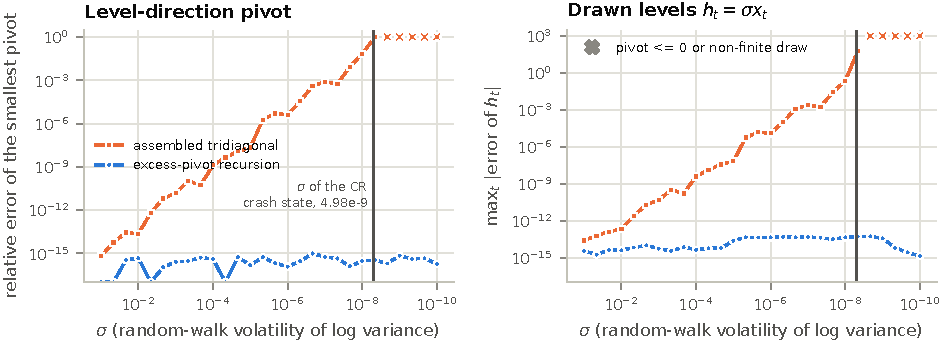
\includegraphics[width=0.8\linewidth]{figures/fig_laplacian_pivots.pdf}
\caption{The random-walk SV path system at small $\sigma$: level-direction pivot and error in
the level of $h$ against $\sigma$, for the assembled factorisation and the excess-pivot recursion,
measured against a 60-digit reference, at the synthetic state of
\code{test_rw_awol_at_a_tiny_sigma} (88 periods), not at the production fit of F2.}
\label{fig:FigE1}
% computed from committed code by docs/paper/figures/make_fig_laplacian_pivots.py (problem() of
% tests/mcmc/blocks/test_sv_core.py); --json docs/paper/data/laplacian_pivots.json writes the plotted numbers
\todo{TODO 23 (author decision): the figure also shows that at $\sigma \le 10^{-8}$, where the
assembled path does not fail, its pivot and the level of $h$ are badly wrong (relative pivot error up
to about 0.95, $h$ off by up to about 61), which \cref{sec:robustness} deliberately does not
state. Keep the figure and state this as a recomputation at a synthetic state, or crop it to the
failing range, and commit the old-path test of TODO 23 either way.}
\end{figure}

\subsection{Performance}\label{app:performance}

Three sources of performance numbers exist in the repository, and only the third measures the
production engine: the stand-in scratch scripts of the design stage (a simplified SV block, data
closed over as constants), the prototypes of the pilot (the real SV block, on a loaded
machine), and the BENCH-P2 baseline of the engine itself through \code{BVAR.fit}.
The paper quotes only the third and never blends them.
% [R] DESIGN section 10.2; docs/phase2/09_pilot.md; tests/bench/baseline.json (dossier 03 section 13.6)
BENCH-P2 fits structural Linear $\times$ SV with fixed hyperparameters to a simulated VAR(4) with SV
($n = 20$, $T = 300$; $k = 81$, $q = 100$, $T_{\mathrm{pad}} = 320$), with 4 chains of 1000 burn-in
and 10,000 kept draws on one CPU device, and times the whole fit, including compilation, storage and
diagnostics, in fresh processes; wall and compilation times are medians over three cold or three
warm runs, and the per-sweep time and peak memory are medians over all six.
% [R] dossier 03 section 13.3 (phase2_perf.summarise)
% [V] benchmarks/phase2_perf.py docstring; tests/bench/test_perf_phase2.py
\cref{tab:TabE2} gives the result recorded at commit deb3929 on an Apple M5 Max that was not
idle (one-minute load 2--6, desktop applications open): 52.3\,s cold and 49.6\,s warm, compilation
3.46\,s cold and 1.00\,s from the persistent cache, 3.90\,ms per sweep, and a peak resident set of
3,043\,MiB.
% [R] tests/bench/baseline.json (deb3929); commit d490730 message
\code{converged} was false in all six runs; according to the commit message, 4 of the 101 primary
quantities missed R-hat 1.01, while every group's minimum bulk ESS exceeded 400.
% [R] baseline.json summary.converged; commit d490730 (R-hat values only in the message)
The slowest-mixing quantities were $\sigma_i$ and $\phi_i$ (minimum ESS per second 10.2 and 11.2),
against about 400 for the own first-lag coefficients.
% [R] baseline.json summary.ess
\cref{tab:TabE3} gives the kernel microbenchmarks at 80 equation--chain lanes, with XLA's flop
and byte counts and the design budget lines: the packed Gram halves the flops of the batched oracle
and is about twice as fast, and the packed Gram, the precision draw and the SV core together take
3.44\,ms of the 3.87\,ms sweep.
% [R] baseline.json kernels; tests/bench/bench_kernels.py (dossier 03 section 13.5 arithmetic)
These figures are from one non-idle machine at one commit and are not portable.
\todo{TODO 9: re-measure BENCH-P2 on an idle machine on the release commit; add an idle x86 entry and,
optionally, the 4-device run.}

\begin{table}[!htbp]
\centering\small
\caption{BENCH-P2 on the production engine: wall time cold and warm, compilation time, time
per sweep, peak RSS, ESS and ESS per second by quantity group, the convergence flag, and the
machine, load and commit.}
\label{tab:TabE2}
% [R] tests/bench/baseline.json (deb3929, non-idle Apple M5 Max); docs/paper/figures/tab_bench.py
\InputIfFileExists{figures/tab_bench.tex}{}{\todo{Generate with \code{tab_bench.py} from
\code{tests/bench/baseline.json}.}}
\end{table}

\begin{table}[!htbp]
\centering\small
\caption{Kernel microbenchmarks at 80 lanes: packed and batched Gram, precision draw, SV
indicators, AWOL draw, exact correction, SV core and sweep; XLA flops and bytes accessed; and the
design budget lines.}
\label{tab:TabE3}
% [R] tests/bench/baseline.json kernels; tests/bench/bench_kernels.py; docs/paper/figures/tab_kernels.py
\InputIfFileExists{figures/tab_kernels.tex}{}{\todo{Generate with \code{tab_kernels.py}.}}
\end{table}

\emph{Not measured on the production engine.}
The 4-device stretch target (only pilot projections exist), the reduced-form CCCM sampler, SV($t$)
and SV with outliers and $t$, Linear $\times$ Constant without dummy rows, and an idle x86 machine;
the only x86 baseline in the history was measured under heavy load on four cores and is labelled
provisional.
% [R] dossier 03 sections 13.7-13.8 (git show d37e059:tests/bench/baseline.json)

\emph{One OpenBLAS thread while chains run.}
On CPU, jaxlib lowers Cholesky factorisations and triangular solves to LAPACK and BLAS calls into
SciPy's library, and XLA already runs those calls on its own threads; the engine therefore restricts
OpenBLAS to one thread while chains run.
The function is a no-op where no OpenBLAS with a thread API is loaded, as on macOS Accelerate, so the
reference baseline did not exercise it.
The claim that results do not depend on the thread count for factors smaller than $128\times128$ is
recorded in the module docstring, not tested; the committed tests check only the set and restore
semantics.
% [V] src/rai_bvar/engines/mcmc/_blas.py; tests/mcmc/runner/test_blas_threads.py; [R] invariance claim (docstring)

\emph{Dense eigen path with dummy rows.}
For Mode~I $\times$ Constant with SOC/SUR rows at $n = 20$, $p = 4$, $T = 300$, the dense eigen path
took 0.46\,ms per sweep against 1.53\,ms for the per-sweep Cholesky, on an Apple M5 Max under a
concurrent load of 3--5; the two paths agree within the path-versus-path envelope of
\cref{sec:validation}.
% [R] timing: NOTES 14 (one run under load); [V] agreement: tests/mcmc/blocks/test_dummies.py::test_dense_eigen_path_with_dummies_*

\subsection{Platform caveats}\label{app:platform}

On macOS with NumPy and SciPy on Accelerate, \code{slogdet} and \code{det} emitted runtime
warnings on two well-conditioned symmetric positive definite tridiagonal matrices of a dense oracle,
which the suite's warning filter turned into failures; the oracle now takes the log-determinant from
the Cholesky factor, and the code under test is unchanged.
% [R] commit dd8244e; issue #3 item 1 (no minimal reproducer committed)
A Phase~1 empirical-Bayes test intermittently crashes the interpreter on the same platform; the root
cause is unknown and it is not tied to the MCMC code.
% [R] issue #3; dossier 05 section 5.7
Linux CI is the reference platform; neither observation is attributed to a particular library.

% -------------------------------------------------------------------------------------
\section{Clark--Ravazzolo supplement}\label{app:cr}
% -------------------------------------------------------------------------------------

This appendix documents the replication of \cref{sec:replication}: the provenance of the
acceptance run, its pre-registration, the criteria and deviations exactly as coded, the run history,
the data and models, and further tables and figures.
Every number of the acceptance run is a placeholder filled from
\code{benchmarks/reports/clark_ravazzolo_acceptance.json}; numbers of the first full run (report
commit 551f181, code 4bb978a, path-conditioned estimator, $4\times5000$ draws) are history only and
are marked as such.
% [ACC] acceptance JSON (to be committed, TODO 2); [FULL] benchmarks/reports/clark_ravazzolo.json (551f181)
Line numbers refer to \code{benchmarks/clark_ravazzolo.py} at commit c823d20.

\subsection{Provenance of the acceptance run}\label{app:cr-provenance}

The acceptance configuration and its pre-registration were committed together in c823d20, before the
run was launched.
According to the run record, the run was started afterwards from a detached worktree at that commit
with a clean working tree,
with the command \code{benchmarks/clark_ravazzolo.py}
\code{benchmarks/reports/clark_ravazzolo_acceptance} \code{--config acceptance} \code{--n-jobs 10} and a fresh score cache named after the commit.
% [R] run record (OUTLINE section 0.4); the run log is ephemeral (TODO 2)
\todo{TODO 2: archive the run log with its UTC start time as evidence that the launch followed
c823d20, and commit \code{clark_ravazzolo_acceptance.\{json,md\}} from the acceptance worktree.}
The script labels a report as the acceptance run only when \code{acceptance_gaps} (l.\,1022) returns
nothing: the configuration must be the registered one (estimator, MCMC budget, forecast draws,
origin and ordering steps, noise replications, backtest seed 0), every stage must have run (the
structural pair and all 24 orderings), and the commit must be known with no uncommitted changes to
tracked files.
% [V] benchmarks/clark_ravazzolo.py l.1022-1060 (acceptance_gaps, is_acceptance); tests/unit/test_clark_ravazzolo_script.py
The acceptance report records \code{config.name} = \acc{config.name}, \code{config.lpd_method} =
\acc{config.lpd_method}, \code{config.draws} = \acc{config.draws}, \code{config.mcmc} =
\acc{config.mcmc}, \code{config.seed} = \acc{config.seed}, \code{versions.git_commit} =
\acc{versions.git_commit} and \code{versions.git_dirty} = \acc{versions.git_dirty}, and whether the
JSON has no \code{pending} key (\acc{absent(pending)}).
The values that \code{acceptance_gaps} requires are \code{"acceptance"}, \code{"integrated"}, 8000,
4 chains $\times$ 20,000 kept draws with burn-in 1000, seed 0, a known commit and
\code{git_dirty} = \code{false}, with no \code{pending} key.
The function does not compare the commit with c823d20; that the run is at c823d20, the commit that
adds the pre-registration, is a requirement of the pre-registration itself and is checked from
\code{versions.git_commit}.
% [V] benchmarks/clark_ravazzolo.py l.186-199 (ACCEPTANCE config), l.207-209 (PREREGISTRATION, PREREGISTERED_SEED,
% REFERENCE_RUN), l.1022-1055 (acceptance_gaps: no comparison of git_commit with a fixed hash)
Two sentences of the repository's ledgers that still said the acceptance configuration ``keeps 1000
forecast draws'' were corrected after the launch, in d58c9ef, which changes documentation only; the
script at c823d20 uses 8000 (l.\,194), as pre-registered.
% [V] git show d58c9ef (docs/paper/NOTES.md, docs/phase2/DESIGN.md only)

\subsection{The pre-registration}\label{app:prereg}

The pre-registration is reproduced below as committed at c823d20, in the file
\code{benchmarks/reports/clark_ravazzolo_preregistration.md}.
Only the typography has changed (Markdown to \LaTeX); the words, numbers and structure are those of
the file.
% [PREREG] c823d20: every number in the quotation below is from the committed pre-registration

\begin{quote}\footnotesize
\textbf{Clark--Ravazzolo replication: pre-registration of the acceptance run}

Written 2026-10-23, before any score of the acceptance run was computed. The acceptance run is
\code{benchmarks/clark_ravazzolo.py} \code{benchmarks/reports/clark_ravazzolo_acceptance} \code{--config acceptance}
with a fresh cache (\texttt{--cache \textasciitilde/.cache/rai-bvar-cr-\textless short
commit\textgreater}; the command is in the script's docstring), on a clean working tree at the commit
that adds this file. The report header records that commit and whether tracked files differ from it;
the report is labelled the acceptance run only when they do not, every stage ran, and the config,
estimator and backtest seed are the ones below. The previous full run (\code{--config full}, report
\code{benchmarks/reports/clark_ravazzolo.md} committed in \code{551f181}) is the reference this
document departs from.

\medskip\noindent\textbf{Why there is a second run}

The full run met criteria 1, 2, 3 and 5 and missed 4 and 6 (N08 \S C5, as coded in
\code{benchmarks/clark_ravazzolo.py}). The two misses had diagnosable causes. Neither was a sign that
SV(rw) loses to Constant.
\begin{itemize}
\item \textbf{Criterion 6} failed only on \code{compare()}'s convergence gate. The SV(rw) verdict was
``better'' in 24/24 orderings with the gate off and 0/24 with it on, because SV(rw) converged at
57--82\% of origins against the 95\% gate.
\item \textbf{Criterion 4} failed on one cell: full-sample UR, $\Delta$LPS(h=8) = +1.954 $>$
$\Delta$LPS(h=1) = +0.159. A handful of 2007--08 origins drive it. There the path-conditioned
Rao--Blackwellised estimator is degenerate: one forecast draw carries all the weight, and the score
is biased low by up to tens of nats, more for the thinner-tailed Constant arm.
\end{itemize}
These changes are motivated by that failure analysis, so the run is not blind to the previous
results. What is pre-registered is that the settings below were fixed before any score of the new
run existed, and that the criteria are evaluated on them as coded, whatever the outcome.

\medskip\noindent\textbf{What changes (and only this)}
\begin{enumerate}
\item \textbf{MCMC budget for every MCMC arm, in every stage:} 4 chains $\times$ 20,000 kept draws,
burn-in 1000, thin 1 (previously 4 $\times$ 5000, burn 1000). With the default \code{store_max = 2500}
the parameters of one in $\lceil 20{,}000 / 2500\rceil = 8$ kept draws are stored (10,000 in all), and
the forecast draws are taken from those; R-hat and ESS use every kept draw.
\begin{itemize}
\item Evidence: fit-level convergence diagnostics only, with no forecasts or scores. The data are the
same and the fit seeds are the CR main-stage ones.
\item SV(rw), identity ordering: 72/106 origins converge at 4 $\times$ 5000; 79/106 with burn 5000;
92/106 with 8 chains; \textbf{106/106 at 4 $\times$ 20,000} (max R-hat 1.0061, min bulk ESS 1763).
\item The two worst orderings of the previous run (INFL $>$ UR $>$ GDP $>$ TBILL and INFL $>$ UR $>$
TBILL $>$ GDP): 71/106 and 63/106 at 4 $\times$ 5000 with the main-stage fit seeds;
\textbf{106/106 and 106/106 at 4 $\times$ 20,000} (max R-hat 1.0049 and 1.0046, min ESS 1689 and
1717). The previous run's ordering stage, which fits each ordering with its own backtest seed, had
63/106 and 60/106 there (and 69/106 for the identity ordering against 72/106 in the main stage), so
this evidence is at the main-stage seeds, not at the ordering stage's.
\item All 520 + 424 diagnostic fits finished without error. Every base-budget failure is on a
$\sigma$ quantity and is marginal (R-hat $<$ 1.03), consistent with R-hat sampling noise at bulk ESS
$\sim$600, not with a stuck sampler.
\end{itemize}
\item \textbf{Primary log predictive density: the path-integrated Rao--Blackwellised estimator}
(\code{lpd_method="integrated"}; DESIGN, the decision row added with it).
\begin{itemize}
\item For h $>$ 1 it conditions each draw on its parameters and its drawn latent scale path only,
and integrates the intermediate y's out analytically.
\item At h = 1 it is identical to the previous estimator.
\item The previous (path-conditioned) estimator is reported as a secondary number in criterion 4's
detail, and per cell in the JSON (\code{dlps_conditioned}, \code{dlpd_conditioned}); it never
enters a rule.
\end{itemize}
\item \textbf{Forecast draws per origin: 8000} (previously 1000), in every stage.
\begin{itemize}
\item Reason: the integrated LPD is exact given each draw but is still an average over draws, and at
crisis origins the weights concentrate on a few of them. In the review of the estimator (2008Q2, UR
h = 8, at the budget of item 1; precision only, no criterion evaluated), Constant's 1000-draw value
sat on average about 0.3--0.6 nats below the 80,000-draw value, with an sd of 0.75--1.06 nats across
thinning offsets. SV(rw)'s varied with sd $\approx$ 1.4 nats across forecast seeds, more than its
MCSE, and its expected bias was as large as Constant's, so the error favours neither arm.
\item With 8000 draws the thinning error dropped to an sd of 0.09--0.19 nats with bias $\approx$ 0.
\item It does not remove the MCMC component: the 80,000-draw values still differ by about 1.3 nats
across fit seeds at that origin.
\item The cost is small next to the fits.
\end{itemize}
\end{enumerate}

\medskip\noindent\textbf{What does not change}
\begin{itemize}
\item \textbf{Data:} FRED-QD/FRED-MD vintage 2026-09 with the same SHA-256 checks, the four series
and their transformations, and the estimation start 1965Q1.
\item \textbf{Models:} Constant(iw\_equivalent), SV(rw), SV, SV(rw,t10), AR-SV(0.9), and the
structural pair. The mean prior is \code{Minnesota(form='reduced',} \code{hierarchy='fixed',} \code{lambda_=0.2,}
\code{alpha=2,} \code{cross=1,} \code{mean=0)} with p = 4.
\item \textbf{SV priors:} the library defaults. CR's own RW-SV $\sigma^2$ prior IG(1/2, 0.0175) is
\textbf{not} adopted. It stays a documented deviation, and adopting it now would be a modelling
change decided after seeing results.
\item \textbf{Origins and horizons:} origins 1985Q1--2011Q2 (106) with the 1985Q1--2007Q4
pre-crisis subset (92); expanding window; horizons 1, 2, 4, 8.
\item \textbf{Seeds:} backtest seed 0, per-origin fit seeds (DESIGN \S 11.6), cold starts; the
ordering stage with all 24 orderings and the same noise replications.
\item \textbf{Rules:} the criteria 1--6 rules and thresholds exactly as coded. That includes the 95\%
convergence gate of \code{compare()} (R-hat $<$ 1.01 and bulk ESS $>$ 400 on every primary quantity)
and the RB-degenerate flag (joint \code{lpd_mcse} $\ge$ 0.9; descriptive only).
\end{itemize}

\medskip\noindent\textbf{Stated in advance}
\begin{itemize}
\item \textbf{Criterion 4 may still fail on UR.} The WP23 review's estimate with corrected tail
origins was UR h = 8 $\approx$ +0.23 against +0.157 at h = 1, which breaks the coded rule
$\Delta$LPS(h=8) $<$ $\Delta$LPS(h=1). If it fails, it is reported as a difference from CR,
attributed with evidence where possible (final vintage instead of real-time data, Chan's
iw\_equivalent baseline, library-default SV priors). It is not tuned.
\item \textbf{Criterion 6} is expected to pass if the convergence gate is met. Its h = 1 scores are
estimator-independent.
\item \textbf{The integrated LPD still carries Monte Carlo error at tail origins} (item 3): about
1.3 nats per arm at a crisis origin from the MCMC itself. That amounts to a few hundredths of a nat
in a 106-origin mean, but it is not zero. The RB-degenerate flag stays descriptive.
\item \textbf{No further run with different settings} is made after this one's scores are seen,
except to fix a bug. A bug fix is documented, and the affected stages are rerun in full with these
settings and a fresh cache (the score-cache keys do not change with the code).
\end{itemize}
\end{quote}

The fit-level diagnostic that the first item cites is not yet committed, so its numbers are those of
the pre-registration (\cref{tab:TabF6}).
\todo{TODO 4: commit the diagnostic script and its output (e.g.\
\code{benchmarks/cr_convergence_diagnostic.py} and \code{benchmarks/reports/cr_convergence_diagnostic.json});
an uncommitted copy of a script and of 520 + 424 fit records sits under
\code{docs/paper/figures/data/convergence_diagnostic/} in the paper worktree.}

\subsection{The criteria as coded}\label{app:cr-criteria}

The six criteria of the replication plan are qualitative; the script turns them into the operational
rules below, which are the project's own choices (for example, ``about 1'' became $\le 1.02$ and
``systematically'' became at least 3 of 4 joint horizons or 8 of 16 cells).
The rules are quoted from the \code{rule} strings of \code{criteria} (l.\,666), with typography
changed only.
% [V] benchmarks/clark_ravazzolo.py l.666-835 (criteria) at c823d20
\begin{enumerate}
\item ``$\Delta$LPS(SV(rw) $-$ Constant) $>$ 0 at h = 1, 2 for all four variables in the full and
pre-crisis samples, and the joint $\Delta$LPD at h = 1 $>$ 0 with one-sided DM/HLN p $<$ 0.10 in both
samples''
\item ``CRPS ratio SV(rw)/Constant $<$ 1 at h = 1, 2 for all four variables (full sample)''
\item ``RMSE ratio SV(rw)/Constant $\le$ 1.02 (`about 1') at h = 1, 2 for all four variables (full
sample); CR's gains for GDP and the bill are 5--10\%''
\item ``full sample: $\Delta$LPS(h=8) $<$ $\Delta$LPS(h=1) for UR and TBILL; pre-crisis:
$\Delta$LPS(h=8) $>$ 0 for GDP and INFL''
\item ``neither SV(rw,t10) nor AR-SV(0.9) is better than both SV(rw) and SV (one-sided DM/HLN p $<$
0.10, positive $\Delta$LPD) at $\ge$ 3 of 4 joint horizons or $\ge$ 8 of 16 marginal cells (full
sample)''
\item ``in every one of the 24 orderings: compare() verdict SV(rw) vs Constant at h = 1 is `better',
and the one-sided DM/HLN p-value of the marginal log score is $<$ 0.10 for GDP and TBILL at h = 1''
\end{enumerate}
Two features of the coded rules are worth stating.
Criterion~4's rule compares the $h = 8$ gain with the $h = 1$ gain only, whereas the qualitative
wording is ``shrinks or turns negative''.
Criterion~6 is met only if the verdict is ``better'' in every ordering both with the convergence gate
on, as \code{compare()} returns it, and with the gate off, and if both $p$-values are below 0.10 in
every ordering.
% [V] l.807: met = not ungated and not dm_fail and not gated
The outcome of each criterion and the numbers behind it are \acc{criteria[*].met} and
\acc{criteria[*].detail}; under the integrated estimator, criterion~4's detail also reports the
path-conditioned values as a secondary number.
% [V] _c4_secondary (l.621, called at l.754)

\subsection{Deviations from the target}\label{app:cr-deviations}

The report prints the following list, quoted from \code{DEVIATIONS} (l.\,1380), followed, for the
integrated estimator, by \code{LPD_INTEGRATED_DEVIATION} (l.\,1372).
References to sections are to the repository's replication plan (N08) and design documents.
% [V] benchmarks/clark_ravazzolo.py l.1372-1402 at c823d20
\begin{enumerate}\small
\item ``Not a deviation from CR, but from the library default: every own-lag prior mean is 0, as in
CR (WP App.~6.1), including the UR and TBILL levels; the library warns that this contradicts their
level transformation codes (it would centre them on 1).''
\item ``Pseudo real time on the final FRED-QD 2026-09 vintage instead of CR's RTDSM real-time
vintages and second-release actuals (D4; \S C2). Score levels differ; rankings are expected to be
robust (\S C6).''
\item ``Estimation starts in 1965Q1, not 1955Q1 (FRED-QD starts in 1959; \S C2).''
\item ``Inflation uses the chain-type GDPCTPI (FRED-QD has no GDPDEF; \S C6).''
\item ``Baseline: Constant(`iw\_equivalent') (Chan 2022) stands in for CR's normal-diffuse VAR
(\S C3); the SV arms use the library's default SV priors except the two CR variants (no prior was
tuned). CR's RW-SV $\sigma^2$ prior IG(1/2, 0.0175) and its 36-observation training prior for $h_0$
are not used (the latter would violate R9, \S C6).''
\item ``AR-SV variant: CR's $a_1 \sim$ N(0.9, 0.05$^2$) is mapped to ($\phi$+1)/2 $\sim$ Beta(71.25,
3.75) (same mean and sd on $\phi$); the SV level $\mu$ keeps the library's in-window data-centred
prior instead of CR's $a_0 \sim$ N(0, 0.4$^2$).''
\item ``LPD: the primary score is the Rao--Blackwellised predictive density; CR's Gaussian
approximation is reported alongside (\S C4, \S C6).''
\item ``Significance: one-sided DM/HLN p-values are descriptive under an expanding window; compare()
therefore decides `better' through the Model Confidence Set (SPEC \S 9.5).''
\item ``compare() turns a verdict `inconclusive' when fewer than 95\% of origins converged
(R-hat/ESS targets of DESIGN \S 8.2); verdicts are reported with that gate on (as returned) and
off.''
\item[] \code{LPD_INTEGRATED_DEVIATION}: ``LPD estimator: the primary score is the library's
path-integrated Rao--Blackwellised estimator (\code{lpd_method='integrated'}, DESIGN \S 7.3, D-34),
not the path-conditioned SPEC \S 7 default; at h = 1 the two are identical, so every h = 1 cell and
criterion 6 (h = 1 only) are estimator-independent. The path-conditioned $\Delta$LPS is reported for
the criterion-4 cells only, as a secondary number (never in a rule).''
\end{enumerate}
The Gaussian-approximation log score of item~7 \citep{adolfson2007forecasting} equals, up to an
additive constant, $-\frac12$ times the Dawid--Sebastiani score, which is proper but not strictly
proper
\citep{dawid1999coherent,gneiting2007strictly}; it is a parity metric only.

\subsection{Run history and the first attempt's crash}\label{app:cr-history}

\cref{tab:TabF1} gives each run with its commit, configuration, machine and load, wall time
and outcome.
In order: a quick run with the library's default MCMC settings ($4\times2000$), on a shared
four-core x86-64 virtual machine, main stage only, labelled as not the acceptance run; the first full
attempt on 8a622c5 ($4\times5000$), which aborted in the SV(rw) ordering stage on F2; the fixes
93f2bcd (failure replay) and f60d736 (excess-pivot recursion); the second full run on 4bb978a, which
contains both fixes and the QR $a$-row draw 3d3f51b, report committed in 551f181; the follow-ups of
an independent review of f60d736 in 4fc0162 (including the random-walk auxiliary likelihood), committed
after the second run had started and therefore not part of it; the path-integrated estimator in
b9c66c0; the pre-registration and acceptance configuration in c823d20; and the acceptance run.
% [R] issue #3 (timestamps 01:34Z-10:44Z on 2026-10-23); commit metadata; report headers;
% [V] git merge-base --is-ancestor: 93f2bcd, f60d736, 3d3f51b in 4bb978a, 4fc0162 not (4bb978a 04:09Z,
% 4fc0162 04:36Z, 551f181 05:16Z); the review found the 656-array set unchanged by 4fc0162 (dossier 06 section 8 item 6)
The second full run took \fullrun{3950\,s} (\fullrun{1.10\,h}) from a fresh cache with six worker
processes, while weekly-tier jobs ran alongside.
% [FULL] clark_ravazzolo.json seconds; [R] stage times and load: issue #3, 05:17Z
It differs from the aborted attempt in 41 files, not only by the fix: the dummy-row work, the QR
$a$-row draw, the replay fix and the random-walk fix all entered between the two, so the second run
is not described as differing ``only by the fix''.
% [R] git diff --stat 8a622c5 4bb978a (dossier 06 section 8, fact-check)
The acceptance run's wall time and stage times are \acc{seconds}; its machine and versions are
\acc{versions}.

The crash of the first attempt unfolded as follows.
After the main stage and the Constant orderings had finished, an SV(rw) fit (reduced form, origin
1987Q2, ordering GDP, TBILL, INFL, UR) raised \code{MCMCNumericalError} in \code{EQ_VOL}, equation 0,
chain 0, at burn-in sweep 318, with code 2001 and pivot 0.
The deterministic replay that should have attached diagnostics itself raised (F3), so the state was
reconstructed by a separate replay, which showed $\sigma = 4.98\times10^{-9}$ for GDP.
The fix f60d736 replaced the assembled factorisation by the excess-pivot recursion, and the second
full run, on 4bb978a, completed all 24 orderings without a crash.
An independent review of f60d736 found no defect; its follow-ups (4fc0162) came after that run had
started and left the 656-array invariance set bitwise unchanged, so the run's report stands.
% [R] issue #3 ("Item 7: the full run crashed" and following comments); commits 93f2bcd, f60d736, 4fc0162;
% [V] tests/mcmc/blocks/test_sv_core.py tiny-sigma tests
\todo{TODO 29: decide whether to say that the committed quick report, which predates f60d736, may
have been affected by the old random-walk path; cite quick-run numbers only as context.}

\begin{table}[!htbp]
\centering\small
\caption{Run history of the replication: commit, configuration, machine and load, wall time
and outcome of each run, from the quick run to the acceptance run.}
\label{tab:TabF1}
% [R] headers of clark_ravazzolo_quick.json and clark_ravazzolo.json (config, versions, seconds); issue #3;
% commit metadata; [ACC] config, versions, seconds; run log (TODO 2); docs/paper/figures/tab_runs.py
% NOTE for tab_runs.py: 4fc0162 is not an ancestor of 4bb978a (full run #2); list it after that run, not among its fixes
\InputIfFileExists{figures/tab_runs.tex}{}{\todo{Generate with \code{tab_runs.py}.}}
\end{table}

\subsection{Data and models}\label{app:cr-data}

\cref{tab:TabF2,tab:TabF3} give the data and the model arms as coded.

\begin{table}[!htbp]
\centering\small
\caption{Data of the replication. Rates are non-annualised quarterly rates; the estimation
sample starts in 1965Q1 (one raw quarter earlier is kept for the difference).}
\label{tab:TabF2}
% [V] benchmarks/clark_ravazzolo.py l.137-144 (VINTAGE, SERIES, ESTIMATION_START, FULL, PRE_CRISIS_END,
% HORIZONS, LAGS), l.236-266 (load_data), l.269-293 (assert_quarterly_averages), l.296-320 (assert_in_window),
% l.1496 (in-window check on the primary arm only)
\begin{tabular}{@{}p{0.10\linewidth}p{0.31\linewidth}p{0.13\linewidth}p{0.38\linewidth}@{}}
\toprule
Variable & CR definition & FRED-QD series & Transformation in the script \\
\midrule
GDP & real GDP growth, $100\,\Delta\log$ & \code{GDPC1} & $100\log$ level, then tcode 2 \\
INFL & inflation in the GDP price index, $100\,\Delta\log$ & \code{GDPCTPI} & $100\log$ level, then tcode 2 (chain-type index; FRED-QD has no deflator series) \\
UR & unemployment rate, quarterly average of monthly values & \code{UNRATE} & level, tcode 1 \\
TBILL & 3-month Treasury bill rate, quarterly average & \code{TB3MS} & level, tcode 1 \\
\midrule
\multicolumn{4}{@{}p{0.96\linewidth}@{}}{\emph{Sample.} Vintage 2026-09 of FRED-QD and FRED-MD,
SHA-256 checked (\cref{app:repro}); estimation from 1965Q1; expanding window; origins
1985Q1--2011Q2 (106) and the pre-crisis subset 1985Q1--2007Q4 (92); horizons 1, 2, 4, 8; $p = 4$.} \\
\multicolumn{4}{@{}p{0.96\linewidth}@{}}{\emph{Run-time checks.} (i) FRED-QD \code{UNRATE} and
\code{TB3MS} equal the within-quarter means of the FRED-MD monthly series of the same vintage
(tolerance 0.01 over more than 200 quarters; first full run: maximum absolute difference
\fullrun{$3.3\times10^{-5}$} over \fullrun{270} quarters; acceptance run: \acc{data_checks.aggregation}).
(ii) No look-ahead: at origins 1985Q1, 2007Q4 and 2011Q2 the resolved prior, hyperparameters and
padded data are bitwise identical when the vintage is cut at the origin, checked for the primary arm
only (\acc{data_checks.in_window}). (iii) The checksums of the vintage files.} \\
\bottomrule
\end{tabular}
\end{table}

The FRED-QD series are those of \citet{mccracken2021fredqd} and the monthly series those of
\citet{mccracken2016fredmd}; the data are downloaded on demand and not bundled.
CR's estimation used real-time vintages \citep{croushore2001realtime}; the replication runs in
pseudo real time on the final vintage, with the start date of \citet{clark2011realtime}.
\todo{TODO 21: confirm the official FRED-QD 2026-09 tcodes of these four series (the script loads
raw levels and sets its own codes), and align \code{fred.py} to cite McCracken and Ng (2021).}

\begin{table}[!htbp]
\centering\footnotesize
\caption{Model arms. Every arm uses the mean block \code{Linear(prior=Minnesota(form="reduced",}
\code{hierarchy="fixed",} \code{lambda_=0.2,} \code{alpha=2.0,} \code{cross=1.0,} \code{mean=0.0))} with $p = 4$, sampled by the
corrected triangular algorithm \citep{carriero2022corrigendum}, except the structural pair, which uses
\code{form="structural"} (Mode~I). SV priors are the library defaults unless stated.}
\label{tab:TabF3}
% [V] benchmarks/clark_ravazzolo.py l.325-350 (minnesota, models, structural_models), l.352-355 (PRIMARY_SV,
% RB_CEILING); src/rai_bvar/components/specs.py (defaults)
\begin{tabular}{@{}p{0.17\linewidth}p{0.30\linewidth}p{0.20\linewidth}p{0.25\linewidth}@{}}
\toprule
Arm & Volatility specification & CR counterpart & Role \\
\midrule
Constant & \code{Constant("iw_equivalent")}, the order-invariant prior of \citet{chan2022asymmetric} & VAR with a normal-diffuse prior & baseline of every relative measure; negative control of the ordering stage \\
SV(rw) & \code{SV(rw=True)}: $h_0 \sim \mathrm{N}(\log(\psi_\iota/\iota), 4)$, $\sigma^2 \sim 0.1\chi^2_1$, in-window & VAR-SV (random walk) & primary arm of criteria 1--4 and 6 \\
SV & \code{SV()}: $\mu \sim \mathrm{N}(\log(\psi_\iota/\iota), 10)$, $(\phi+1)/2 \sim \mathrm{Beta}(20, 1.5)$, $\sigma^2 \sim \chi^2_1$ & --- & second reference of criterion 5 \\
SV(rw,t10) & \code{SV(rw=True, tails="t", nu_prior=DiscreteUniform(10, 10), t_scale="unit")} & VAR-SVt with $d = 10$ & criterion 5 variant; $\nu$ fixed, so its grid-bound warning fires by design \\
AR-SV(0.9) & \code{SV(phi_prior=Beta(71.25, 3.75))} & VAR-ARSV with $a_1 \sim \mathrm{N}(0.9, 0.05^2)$ (same mean and sd on $\phi$) & criterion 5 variant \\
Constant / SV(rw) [structural] & \code{Constant("ig")} / \code{SV(rw=True)} in structural Mode~I & --- & robustness pair \\
\bottomrule
\end{tabular}
\end{table}

CR's target is \citet{clark2015macroeconomic}; the numbers compared are those of the working paper's
Tables~1--3 \citep{clark2012macroeconomic}, as hard-coded in the script (\code{CR_FULL}, l.\,147;
\code{CR_PRE_DLPS}, l.\,167).
\todo{TODO 22: obtain the JAE tables, or keep saying that the working-paper numbers are used; resolve
the 40-versus-56 count of re-read numbers in N08.}
CR's VAR uses a Minnesota prior with $\theta = 0.2$, $1/l^2$ decay and a normal-diffuse prior on
the coefficients \citep{kadiyala1997numerical}; their VAR-SV samples random-walk log-volatilities by
the single-move step of \citet{jacquier1994bayesian}, with a $\sigma^2$ prior
$\mathrm{IG}(1/2, 0.0175)$ that the replication does not adopt.
The working paper does not state a variable ordering, which is why all 24 orderings are run.
% [R] dossier 06 section 2 (N08 sections C2, D item 2; the JAE text was not accessible)

\subsection{Further results of the acceptance run}\label{app:cr-results}

\cref{tab:TabF4} gives the pre-crisis comparison of SV(rw) and Constant at $h = 1$ and $h = 8$,
\cref{tab:TabF5} every SV arm against Constant with the convergence shares, the verdicts with
the gate on and off, the route by which each verdict was reached and the variant comparisons of
criterion~5, and \cref{tab:TabF7} the Constant arm's levels against CR's benchmark VAR together
with the compute record.
The reading rules of \cref{sec:replication} apply to every number here.
Under the expanding window, any ``better'' verdict can only come through the model confidence set
\citep{hansen2011model}.
In the first full run the pre-crisis GDP $h = 8$ cell, which criterion~4 needs to be positive, was
\fullrun{$+0.108$} under the path-conditioned estimator and \fullrun{$-0.004$} under the Gaussian
approximation; its acceptance values are \acc{relative.pre_crisis['SV(rw)'].variables.GDP['8'].dlps} and
\acc{relative.pre_crisis['SV(rw)'].variables.GDP['8'].dlps_gauss}.
% [FULL] relative.pre_crisis['SV(rw)'] (551f181); [ACC]
The fit-level diagnostic covered only SV(rw), and only three of the 24 orderings at the main-stage
seeds, so the gate-on verdicts of SV, SV(rw,t10) and AR-SV(0.9) may stay inconclusive.
% [PREREG] item 1

\begin{table}[!htbp]
\centering\small
\caption{Pre-crisis sample (1985Q1--2007Q4), SV(rw) against Constant at $h = 1$ and $h = 8$:
$\Delta$LPS under the integrated (primary) and the path-conditioned estimator, the
Gaussian-approximation $\Delta$LPS and the number of RB-degenerate origins, with CR's working-paper
values.}
\label{tab:TabF4}
% [ACC] relative.pre_crisis['SV(rw)']; CR_PRE_DLPS (l.167); docs/paper/figures/tab_cr_precrisis.py
\InputIfFileExists{figures/tab_cr_precrisis.tex}{}{\todo{Generate with \code{tab_cr_precrisis.py} from
the acceptance JSON.}}
\end{table}

\begin{table}[!htbp]
\centering\small
\caption{All SV arms against Constant: joint $\Delta$LPD by horizon, share of converged
origins, the \code{compare()} verdict with the gate on and off and its route (DM or MCS), MCS
membership; and the variant comparisons of criterion~5, full and pre-crisis samples.}
\label{tab:TabF5}
% [ACC] relative.{full,pre_crisis}[arm].joint, converged.{full,pre_crisis}, verdicts.{full,pre_crisis},
% variants[variant][ref].joint; docs/paper/figures/tab_cr_arms.py
\InputIfFileExists{figures/tab_cr_arms.tex}{}{\todo{Generate with \code{tab_cr_arms.py} from the
acceptance JSON.}}
\end{table}

\begin{table}[!htbp]
\centering\small
\caption{Constant-arm levels against CR's benchmark VAR at $h = 1$ (average log score and RMSE), and
the compute record of the acceptance run: machine, number of worker processes, stage times and wall
time. The two log-score rows use different estimators and data vintages, so this is a sanity
check, not a parity test.}
\label{tab:TabF7}
% [ACC] relative.full['SV(rw)'].variables[v]['1'].{lps_base,rmse_base}, seconds, versions, config;
% CR levels from N08 section C5; docs/paper/figures/tab_cr_levels_compute.py
\InputIfFileExists{figures/tab_cr_levels_compute.tex}{}{\todo{Generate with
\code{tab_cr_levels_compute.py}; stage times must be written to the JSON or the report.}}
\end{table}

\begin{figure}[!htbp]
\centering
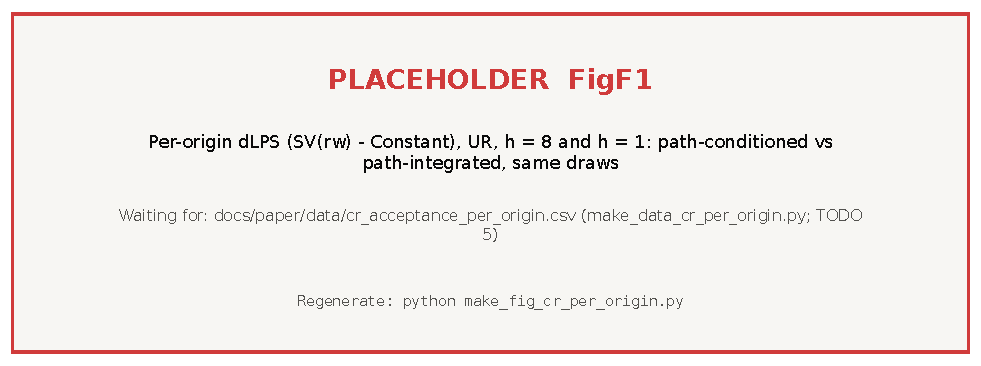
\includegraphics[width=0.9\linewidth]{figures/fig_cr_per_origin.pdf}
\caption{Per-origin $\Delta$LPS of SV(rw) against Constant for unemployment at $h = 8$ (and $h = 1$
for contrast), origins 1985Q1--2011Q2: path-conditioned against path-integrated, from the same
forecast draws of the acceptance run.}
\label{fig:FigF1}
% [ACC] needs docs/paper/data/cr_acceptance_per_origin.csv (TODO 5); docs/paper/figures/make_fig_cr_per_origin.py
\end{figure}
\todo{TODO 5: export the per-origin scores of the acceptance run to
\code{cr_acceptance_per_origin.csv} in \code{docs/paper/data/}, or drop \cref{fig:FigF1,fig:FigF3}.}

\begin{figure}[!htbp]
\centering
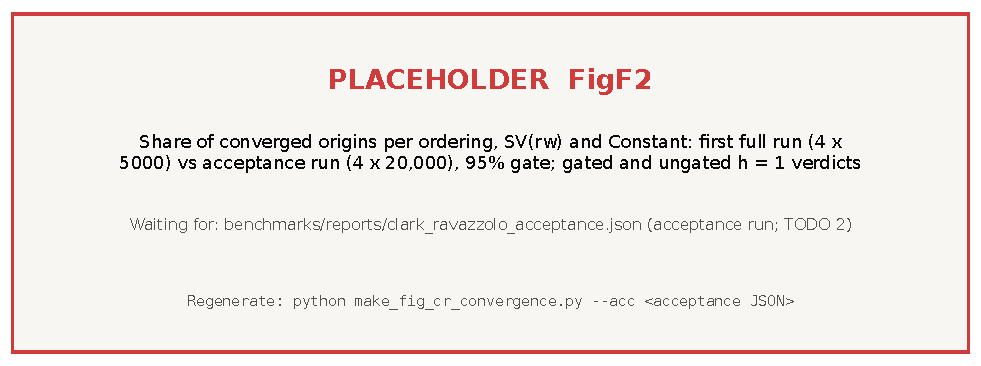
\includegraphics[width=0.9\linewidth]{figures/fig_cr_convergence.pdf}
\caption{Share of converged origins per ordering for SV(rw) and Constant: first full run ($4\times5000$)
against the acceptance run ($4\times20{,}000$), with the 95\% gate; gated and ungated $h = 1$ verdicts
are marked.}
\label{fig:FigF2}
% [FULL] clark_ravazzolo.json orderings.per_ordering[*]; [ACC] orderings.per_ordering[*].{converged_sv,
% converged_constant, verdict_h1, verdict_h1_ungated}; docs/paper/figures/make_fig_cr_convergence.py
\end{figure}

\begin{figure}[!htbp]
\centering
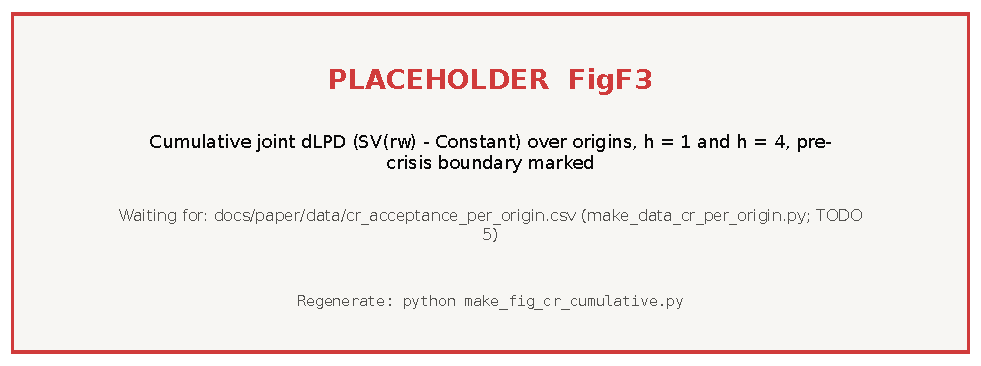
\includegraphics[width=0.9\linewidth]{figures/fig_cr_cumulative.pdf}
\caption{Cumulative joint $\Delta$LPD of SV(rw) against Constant over origins at $h = 1$ and $h = 4$,
with the end of the pre-crisis sample marked.}
\label{fig:FigF3}
% [ACC] needs the per-origin export (TODO 5); docs/paper/figures/make_fig_cr_cumulative.py
\end{figure}

\subsection{Convergence against the MCMC budget}\label{app:cr-budget}

\cref{tab:TabF6} gives the fit-level convergence diagnostic that set the acceptance budget: SV(rw)
fits at the main-stage fit seeds, with no forecasts or scores, at $4\times5000$, with burn-in 5000,
with 8 chains and at $4\times20{,}000$, for the identity ordering and the two worst orderings of the
first run, together with the main-stage against ordering-stage seed comparison.
Its numbers are those of the pre-registration until the diagnostic is committed.
\cref{fig:FigF2} compares the converged shares per ordering of the first full run and the
acceptance run.
The seed comparison is itself evidence of R-hat noise at the threshold: the same models in the same
ordering converged at \fullrun{72} (main-stage seeds) and \fullrun{69} (ordering-stage seeds) of 106
origins, with joint $h = 1$ $\Delta$LPD of \fullrun{$+0.809$} and \fullrun{$+0.838$}.
% [FULL] converged.full['SV(rw)'] = 72/106; orderings.per_ordering[0]; [PREREG] item 1

\begin{table}[!htbp]
\centering\small
\caption{Convergence against the MCMC budget for SV(rw), fit-level only: $4\times5000$, burn-in
5000, 8 chains and $4\times20{,}000$; identity ordering and the two worst orderings; converged
origins, maximum R-hat and minimum bulk ESS; and the main-stage against ordering-stage seed
comparison.}
\label{tab:TabF6}
% [PREREG] benchmarks/reports/clark_ravazzolo_preregistration.md item 1 (c823d20); TODO 4;
% docs/paper/figures/tab_cr_budget.py
\InputIfFileExists{figures/tab_cr_budget.tex}{}{\todo{Generate with \code{tab_cr_budget.py}; the
numbers stay [PREREG] until TODO 4 is done.}}
\end{table}

\subsection{The first full run (history)}\label{app:cr-first-run}

\cref{tab:TabF8} reproduces the first full run's tables for the record: the headline and
pre-crisis comparisons, all arms, the variants, the structural pair, the RB-degenerate origins and
the cells in which the RB and Gaussian $\Delta$LPS differ in sign.
They were produced by the path-conditioned estimator with $4\times5000$ draws and 1000 forecast
draws, and they are history, not results; \cref{sec:replication} summarises what they
showed and why the acceptance run differs.
Across all SV arms and both samples, the RB and Gaussian $\Delta$LPS differed in sign in \fullrun{28}
marginal and \fullrun{8} joint cells, all at $h \ge 2$.
% [FULL] clark_ravazzolo.json rb_gauss_disagree (551f181); dossier 06 section 7.2 (fact-checked)
The order-invariant Constant arm was flagged ``material'' by the ordering diagnostic at two $h > 1$
cells (joint $h = 2$ and UR $h = 8$), with a noise floor resting on one
replicate; this is reported as a limitation of the diagnostic, and the acceptance run's flag is
\acc{orderings.results.Constant.material}.
% [FULL] orderings.results['Constant'].material = True; TODO 26
Differences from CR's levels, such as inflation gains of \fullrun{1.6--3.2} times CR's, are not
attributed to any single cause; final-vintage chain-type prices and the iw\_equivalent baseline are
hypotheses only.

\begin{table}[!htbp]
\centering\small
\caption{First full run, for the record: code 4bb978a, report 551f181, path-conditioned RB
estimator, $4\times5000$ kept draws, 1000 forecast draws. Headline, pre-crisis, all arms, variants,
structural pair, RB-degenerate origins and the RB/Gaussian sign-disagreement cells. These numbers
are history, not results.}
\label{tab:TabF8}
% [FULL] benchmarks/reports/clark_ravazzolo.json (551f181); docs/paper/figures/tab_first_run.py
\InputIfFileExists{figures/tab_first_run.tex}{}{\todo{Generate with \code{tab_first_run.py} from the
first full run's JSON.}}
\end{table}

\clearpage

% -------------------------------------------------------------------------------------
\section{Reproducibility record}\label{app:repro}
% -------------------------------------------------------------------------------------

\emph{Release.}
Every table and figure of the paper is to be regenerated on one release commit of
\pkg{rai-bvar}, whose hash, tag and archive are given here.
\todo{TODO 20: merge \code{phase-2-cr-acceptance} into \code{main}, fix the release commit hash, tag
the release, mint a Zenodo DOI for the release and the replication outputs, add the repository URL,
and re-run \code{ex_a.py} and \code{ex_b.py} on that commit.}

\emph{Validation records.}
With \code{RAI_BVAR_VALIDATION_RECORD} set to \code{docs/paper/data/release}, three test modules
append one JSON line per run to that directory: \code{geweke.jsonl} from \code{tests/geweke}, for
every Geweke tier (G-small, the block configurations, G-full and the recorded \code{exact=False}
rows, distinguished by a \code{tier} field), \code{sbc.jsonl} from \code{tests/sbc} and
\code{mutation.jsonl} from \code{tests/mutation}.
The release record is planned to add the x86-64 mutation record (under a separate name), the
composition-level Tier~B, parity (\code{pytest -m parity_long}) and analytic-twin results, for
which no record hook exists yet and pytest's JUnit XML is the fallback; \code{collect.txt} with
\code{pytest --collect-only -q} and its per-marker variants; and \code{env.json} with the
environment of \cref{tab:TabG2}.
% [V] git grep RAI_BVAR_VALIDATION_RECORD at d58c9ef: tests/geweke/test_geweke_compositions.py (record("geweke", ...)
% for tiers G-small, G-small-block, G-full, G-full-inexact), tests/sbc/test_sbc_compositions.py (sbc.jsonl),
% tests/mutation/test_mutants.py (mutation.jsonl); none in tests/sbc/test_block_tier.py, tests/parity, tests/analytic;
% [REL] the files themselves
\todo{TODO 7: run and commit these records, adding record hooks (or JUnit capture) for composition-level
Tier~B, parity and the twins. Uncommitted Geweke (block, G-full, \code{exact=False}), SBC and
mutation records of unknown commit and machine sit under
\code{docs/paper/figures/data/validation_record/}; they are not release records.}

\emph{Data.}
The FRED vintages are downloaded on demand from the St.\ Louis Fed, verified against the SHA-256
checksums of the package's registry, and cached; they are not bundled.
\begin{center}\footnotesize
\begin{tabular}{@{}ll@{}}
\toprule
Dataset, vintage & SHA-256 of the published file \\
\midrule
FRED-MD 2026-09 & \texttt{d6e239038afbdbf4667c2a63c13c942817bc196fedab4355cd7e0d353ecdd65d} \\
FRED-QD 2026-09 & \texttt{a144b1547ddbad5c68fc934c90c0c0f9837a5139571ba8e64afcc2637aaa3feb} \\
\bottomrule
\end{tabular}
\end{center}
% [V] src/rai_bvar/datasets/fred.py l.71-74 (REGISTRY), unchanged between 62d15f6 and c823d20

\emph{Regeneration.}
The \code{Makefile} in \code{docs/paper} regenerates the figures from committed code and data
(\code{make figures}) and builds the paper (\code{make}); each figure script names its data source
in its header, and \cref{tab:TabG2} is to give the command for each float.
The acceptance tables and figures need \code{benchmarks/reports/clark_ravazzolo_acceptance.json},
and \cref{fig:FigF1,fig:FigF3} the per-origin export of TODO~5.
\todo{TODO 20: the table generators named in the captions (\code{tab_*.py}) are not written yet;
add them to the \code{Makefile}, then state the one command and its wall time on the release
commit.}

\emph{What reproduces how.}
\cref{tab:TabG1} states each guarantee with its scope.
Three levels must be kept apart.
Bitwise equality holds for the listed variations within one platform and one version set, and part
of it is established only with the runner's test doubles (``toys''), not with the production
kernels.
Equality to rounding holds where XLA vectorises the reductions of the production SV and CCCM kernels
differently for different batch sizes: chains are then equal only until a last-bit difference flips
an accept/reject decision, and in distribution afterwards.
Nothing is guaranteed across platforms (OpenBLAS against Accelerate), JAX versions or PRNG
implementations.
% [V] DESIGN section 5.6 with the Stage 2 amendment; dossier 03 section 10
In practice, on one machine and version set, re-runs reproduced the printed output of the analytic
listing of \cref{sec:walkthrough} line for line, that of the MCMC listing except its timing
lines, and the fixed-seed validation statistics to every printed digit; across machines the
mutation statistics agreed to two or three significant figures, and MCMC results can be compared
only within Monte Carlo error.
% [V] dossier 02 section 19 (fact-check re-runs of ex_a.py and ex_b.py); dossier 04 (G-small and mutation re-runs);
% [R] cross-machine mutation statistics (mutants.py EVIDENCE header)

\begin{table}[!htbp]
\centering\footnotesize
\caption{Reproducibility matrix: for a fixed specification, data, seed and device count, each
variation, the guarantee, the test that establishes it, and its scope. ``Toys'' are the runner's
test doubles in \code{tests/mcmc/runner/toys.py}, which implement the block protocols but are not
the production kernels.}
\label{tab:TabG1}
% [V] dossier 03 section 10 (fact-checked at 62d15f6); the test IDs are checked against
% pytest --collect-only by docs/paper/figures/tab_reproducibility.py
\begin{tabular}{@{}p{0.34\linewidth}p{0.26\linewidth}p{0.27\linewidth}c@{}}
\toprule
Variation & Guarantee & Scope & Tests \\
\midrule
chunk size and burn-in piece size & bitwise & toys; production follows from the key layout [TC] & a \\
thinning with aligned sweeps & bitwise & toys & b \\
fused against unfused plan & bitwise & toys (3 configurations) & c \\
\code{vmap} over chains against a sequential loop & bitwise & toys & d \\
chain-count prefix, \code{chains="map"} & bitwise & toys and production \code{structural_sv} & e \\
chain-count prefix, \code{chains="vmap"} & toys: bitwise on macOS, to rounding on x86 Linux; production: rtol $10^{-9}$ & toys; production SV and CCCM kernels, short runs & f \\
\code{vmap} against \code{shard_map} over 4 devices & toys: rtol $10^{-12}$; production: rtol $10^{-9}$ & toys; production \code{structural_sv}, short burn-in & g \\
leading fit axis against looped fits & rtol $10^{-10}$ & toys & h \\
in-loop against post-hoc forecasts & $10^{-12}$ & production & i \\
memory-mapped against in-memory store & equal & toys & j \\
OpenBLAS thread count (factors $< 128\times128$) & bitwise & recorded (module docstring) & --- \\
adding the dummy-row code, with no rows & bitwise (537 arrays) & recorded, one machine; structural test & k \\
platform, JAX version, PRNG implementation, partitionable threefry, spec fields & none & by design & --- \\
\bottomrule
\end{tabular}

\medskip
\begin{minipage}{\linewidth}\footnotesize\raggedright
Tests in \code{tests/mcmc/}:
(a) \code{runner/test_chunking.py::test_chunk_and_burn_piece_size_invariance};
(b) \code{runner/test_chunking.py::test_thinning_with_aligned_sweeps};
(c) \code{runner/test_sweep.py::test_fused_equals_unfused_bitwise};
(d) \code{runner/test_sweep.py::test_vmap_over_chains_equals_sequential_loop};
(e) \code{runner/test_chunking.py::test_chain_prefix_invariance_with_mapped_chains},
\code{::test_mapped_chains_production_prefix};
(f) \code{runner/test_chunking.py::test_chain_prefix_invariance},
\code{::test_production_chain_prefix_with_vmapped_chains_to_rounding},
\code{::test_production_chain_prefix_with_vmapped_reduced_form_to_rounding};
(g) \code{runner/test_devices_bitwise.py::test_shard_map_matches_vmap_in_subprocess};
(h) \code{runner/test_runner.py::test_fit_axis_equals_looped_fits};
(i) \code{forecast/test_forecast_core.py::test_in_loop_forecast_equals_post_hoc_sv},
\code{::test_in_loop_forecast_equals_post_hoc_constant},
\code{::test_in_loop_forecast_equals_post_hoc_with_thinned_storage};
(j) \code{runner/test_storage.py::test_memmap_store_equals_memory_store};
(k) \code{blocks/test_dummies.py::test_dummy_path_is_closed_without_dummies}.
\end{minipage}
\end{table}

Every MCMC fit records the information needed to reproduce it: the \pkg{jax} and \pkg{jaxlib}
versions, the PRNG implementation and whether threefry is partitionable, the platform, device count
and chain method, the seed and the data salt, the resolved Gram mode, constant-volatility path and
$T_{\mathrm{pad}}$, the mixture, offset and exact flag, the ordering, the specification hash and the
package version; the sweep range and the burn-in, draws and thinning are stored with the draws.
% [V] src/rai_bvar/engines/mcmc/results.py _metadata l.140-192, l.247; runner.run_chains l.1123
Keys are counter-based \citep{salmon2011parallel}, derived by \code{fold_in} over seed, stream, data
salt, chain, absolute sweep, block, equation and sub-draw, with uint32 counters and no key in any loop
carry, so draws cannot depend on chunking, burn-in pieces or thinning alignment; with partitionable
threefry, the words drawn directly from a parent key equal the key data of its \code{fold_in}
children, which JAX's key-reuse checker cannot see, and the engine avoids this by giving every
consumer its own sub-key.
% [V] src/rai_bvar/engines/mcmc/keys.py; tests/mcmc/runner/test_sweep.py::test_counter_must_be_uint32;
% tests/mcmc/blocks/test_robust.py::test_ahead_and_transition_give_the_core_its_own_sub_key

\begin{table}[!htbp]
\centering\small
\caption{Environment and regeneration record: versions of Python, NumPy, SciPy, \pkg{jax} and
\pkg{jaxlib}, \pkg{scoringrules} and the BLAS backend; the machines; the release commit; and the
command that regenerates each table and figure.}
\label{tab:TabG2}
% [REL] docs/paper/data/release/env.json (written by docs/paper/figures/run_examples.py);
% docs/paper/figures/tab_environment.py
\InputIfFileExists{figures/tab_environment.tex}{}{\todo{Generate with \code{tab_environment.py} on the
release commit.}}
\end{table}

% -------------------------------------------------------------------------------------
\section{Licensing and source-reading practice}\label{app:licensing}
% -------------------------------------------------------------------------------------

\pkg{rai-bvar} is released under the Apache License 2.0.
% [V] LICENSE; pyproject.toml
The package's practice with respect to GPL-licensed reference software is stated in these words:
\begin{quote}
No code was translated from GPL sources. Algorithms were implemented from the published papers. GPL
packages were run as numerical oracles, and in a few documented cases (named in the repository
notes) their source was read to pin down an oracle's behaviour, defaults or constants, never to write
implementation code.
\end{quote}
% [V] wording: dossier 01 section 6.2 (fact-checked against the notes listed in Table H.1)
\cref{tab:H-notes} lists the repository notes in which GPL or unlicensed source was read, with
the versions and the purpose each note records, and the notes in which none was read.
The versions in the table are those of the source that was read; the parity fixtures were produced
with \pkg{stochvol} 3.2.1 and R \pkg{BVAR} 1.0.5 (\cref{app:parity}).
% [R] tests/parity/SV_PARAMETRIZATION.md "Versions"; DESIGN section 9.9 names stochvol 3.2.9

\begin{table}[!htbp]
\centering\footnotesize
\caption{Repository notes and the reading of third-party source they record.}
\label{tab:H-notes}
% [V] docs/phase2/02_sv_sampler.md l.6, l.597-598, l.608; 01_omori_mixture.md l.9-11; 03_sv_outliers_t.md l.7-9;
% 07_jax_patterns.md l.736, l.764; tests/parity/BVAR_PARAMETRIZATION.md l.3-13; SV_PARAMETRIZATION.md l.9-11;
% 04_cccm_corrected.md l.5; 05_structural_equation_sampler.md l.4; 06_validation_geweke_sbc.md l.3; 08_common_sv_and_ordering.md l.13
\begin{tabular}{@{}p{0.33\linewidth}p{0.60\linewidth}@{}}
\toprule
Note & What was read, and for what \\
\midrule
\multicolumn{2}{@{}l}{\emph{Notes in which source was read}} \\
\code{docs/phase2/02_sv_sampler.md} & \pkg{stochvol} (GitHub sources and CRAN manuals), and the \pkg{bayesianVARs} 0.1.8 and \pkg{bvarsv} 1.1 sources, in the note itself; \pkg{stochvol} 3.2.9, \pkg{bayesianVARs} 0.1.8 and \pkg{bvarsv} 1.1 in its cross-check; read only for published defaults, constants and behaviour; no code transcribed \\
\code{docs/phase2/01_omori_mixture.md} & six GPL packages opened only to confirm the published mixture constants and observable behaviour (which table, which offset, whether a shift is applied) \\
\code{docs/phase2/03_sv_outliers_t.md} & greps of the \pkg{stochvol} C++ and R sources (the $\nu$ proposal, the update order, the $t$ scaling of the simulator), and greps of the replication code of \citet{carriero2024addressing}, which carries no licence (prior constants, outlier grid, mixture table, the $\nu$ log-likelihood constant) \\
\code{docs/phase2/07_jax_patterns.md} & in the cross-check, one \pkg{stochvol} header searched only for the 10 published mixture constants \\
\code{tests/parity/BVAR_PARAMETRIZATION.md} & R \pkg{BVAR} 1.0.5 sources and the JSS article, read to establish the behaviour of the oracle; ``not a description of code to be ported'' \\
\midrule
\multicolumn{2}{@{}l}{\emph{Notes in which no GPL source was read}} \\
\multicolumn{2}{@{}p{0.95\linewidth}@{}}{\code{tests/parity/SV_PARAMETRIZATION.md} (packages only run; behaviour from manuals and experiments); \code{docs/phase2/04_cccm_corrected.md}; \code{docs/phase2/05_structural_equation_sampler.md}; \code{docs/phase2/06_validation_geweke_sbc.md}; \code{docs/phase2/08_common_sv_and_ordering.md}.} \\
\bottomrule
\end{tabular}
\end{table}

The committed parity fixtures that the R oracles produced (in \code{tests/parity/fixtures/}) are
outputs of GPL programs run as oracles; the project treats them as data, not code.
% [V] r_bvar_*.json, stochvol_*.nc, bvars_swa_*.nc (the last from an R script that calls stochvol); the
% .csv inputs in the same directory are data, not oracle output
\todo{TODO 17: decide whether to cite \citet{fsf2026gplfaq} for this position (as a web page, not
legal advice).}
The Bank of England \pkg{bvar} package \citep{labonne2026bvar} is MIT-licensed.
FRED-MD and FRED-QD \citep{mccracken2016fredmd,mccracken2021fredqd} are downloaded on demand and
never bundled, because some series are third-party copyrighted; the named variable sets of the
loader, and the committed fixtures, use only U.S. federal-agency series.
% [V] src/rai_bvar/datasets/fred.py docstring; SPEC section 5.8 (decision D4)

% -------------------------------------------------------------------------------------
\section{Design-review errata relevant to numerics and reproducibility}\label{app:errata}
% -------------------------------------------------------------------------------------

The Phase~2 design was reviewed before implementation, and its errata table maps each of the 28
findings of the reviews (E1--E28) to its resolution.
Four of those that concern numerics and reproducibility are listed below; each was found in the
proposals and resolved in the design before the code it concerned was written.
% [V] docs/phase2/DESIGN.md section 0.2; NOTES C.11
\begin{description}\small
\item[E7] The counter $it_0 + j\cdot\mathrm{thin} + r$ promotes to int64 under 64-bit mode. All counters are uint32 with explicit casts, \code{step_key} raises on any other counter type, and the host checks that the sweep count stays below $2^{32}$ (\cref{alg:C-driver}).
% [V] tests/mcmc/runner/test_sweep.py::test_counter_must_be_uint32
\item[E9] An earlier proposal validated the samplers with the blocks' own prior samplers and log priors. The design adopted an independent reference registry with separate owners, which became the two-implementation rule of \cref{sec:validation}.
% [V] tests/validation/test_log_joint.py::test_references_never_import_kernels
\item[E14] Two ``runtime'' settings, the Gram mode and padding to a maximum length, were not bitwise-neutral. The Gram mode is now resolved by a fixed shape rule and stored in the specification, there is no padding to a maximum, and \code{Runtime} holds only settings that have an invariance test, bitwise except for the device count, which is to rounding (\cref{tab:TabG1}).
\item[E23] $2\log|e_t|$ is $-\infty$ on padded rows and produced NaN. The residual is masked before the logarithm (\cref{alg:C-vol}).
\end{description}
The review process is described in \cref{app:process}; the generic lessons for other
implementations are in \cref{sec:robustness}.

% -------------------------------------------------------------------------------------
\section{Development process and AI-assistance disclosure}\label{app:process}
% -------------------------------------------------------------------------------------

\todo{TODO 30: the author writes and approves this appendix, including the AI-assistance statement,
worded to arXiv policy and to the target venue's; an AI system is not an author.}
The following facts about the process are recorded in the repository and may be used.
The Phase~2 design was produced from three competing proposals (correctness-first,
performance-first and extensibility-first), ranked by two independent reviews (``judges''); the
highest-ranked proposal was taken as the base and elements of the other two were grafted onto it, and
every technical error either review listed was mapped to a resolution (errata E1--E28,
\cref{app:errata}).
% [V] docs/phase2/DESIGN.md front matter and section 0.2
The implementation was split into work packages with separate owners, under the two-implementation
rule: the references of the validation harness were written by packages that wrote no kernel (one
later reference, for the SOC/SUR dummy rows, was written by the kernels' owners from the model;
\cref{sec:validation-harness}), and a test enforces that no reference imports a kernel
module.
% [V] DESIGN section 9.1 (D-22); tests/validation/test_log_joint.py::test_references_never_import_kernels
Independent review runs on x86-64 Linux re-executed parts of the validation suite, including the
mutation suite, and caught further injected errors.
% [R] tests/mutation/mutants.py EVIDENCE header; NOTES 15
\todo{TODO 30: state how AI assistance was used (design, implementation, review, the dossiers and
drafting of this paper), who verified what, and the authorship and acknowledgements.}

% -------------------------------------------------------------------------------------
% Appendix K (TODO for the author) is kept out of the compiled paper: it mirrors OUTLINE.md section 16.
% -------------------------------------------------------------------------------------
\iffalse
\section{TODO for the author}\label{app:todo}
See docs/paper/OUTLINE.md, section 16 (items 1--33). This block is never compiled.
\fi
